\documentclass[12pt]{article}
\usepackage{amsmath}
\usepackage{subcaption}
\usepackage{fontspec}
\usepackage{booktabs}
\usepackage{graphicx}
\usepackage{geometry}
\usepackage{float}
\usepackage{multirow}
\usepackage{array}
\geometry{a4paper, margin=1in}
\usepackage{setspace}
\onehalfspacing
\usepackage{fancyhdr}
\pagestyle{fancy}
\fancyhead{}
\fancyfoot[C]{\thepage}
\usepackage{ctex}
\usepackage{algorithm}
\usepackage{algpseudocode}
\usepackage{hyperref}
\hypersetup{colorlinks=true, linkcolor=blue, citecolor=blue}

% 图片路径
\graphicspath{{../results/}{../results/report_figures/}{../data/}}

\title{\textbf{基于显著特征提取的图像匹配与全景拼接}}
\author{学号：2023010916 \quad 姓名：张章}
\date{\today}

\begin{document}

\maketitle

% ============================================================
\section{引言}

\begin{figure}[H]
\centering
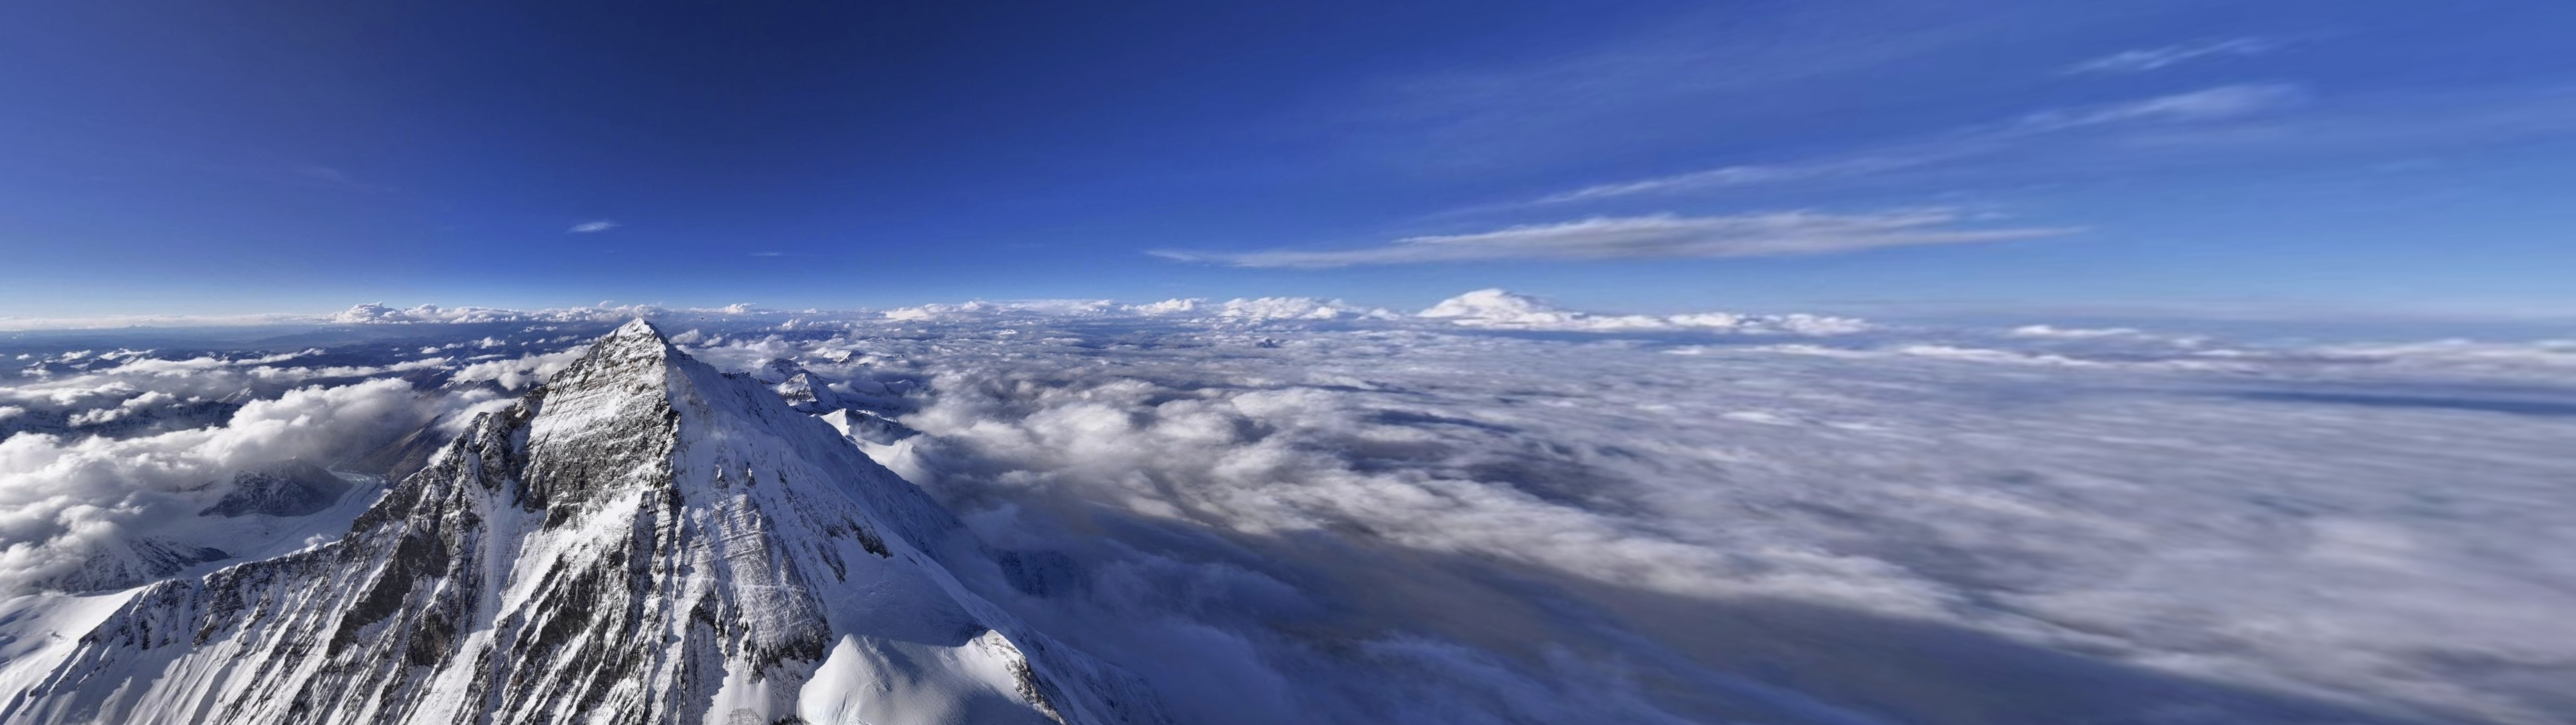
\includegraphics[width=\textwidth]{Everest_stitched.jpg}
\caption{一览众山小。}
\label{fig:stitch_everest}
\end{figure}

本报告为计算机视觉课程中期作业，实现了基于特征点的图像匹配与全景拼接系统。系统包含以下核心模块：(1) Harris角点检测与SIFT特征检测；(2) SIFT与ORB两种特征描述子；(3) SSD距离与比值检验两种匹配策略；(4) 基于RANSAC的单应性矩阵估计与图像拼接。

本文将详细描述各模块的算法原理与实现细节，并通过在9对图像上的实验结果对不同方法进行定量比较与分析。

% ============================================================
\section{图像数据集构建}

\subsection{数据集概述}

本实验共使用9对图像。其中1对为教师提供的标准测试图像（校园建筑场景），3对来自Tanks and Temples公开数据集（Auditorium、Caterpillar、Church），另外5对由作者从Google Earth平台中的街景功能截取（GreatWall、BigBen、Antarctica、Honolulu、Everest）。所有自采集图像均经过统一的16:9比例裁剪，并确保同一对内两幅图像具有相同的分辨率，以保证实验条件的一致性。

\subsection{数据集详细信息}

\begin{table}[H]
\centering
\caption{图像数据集详细信息}
\label{tab:dataset}
\begin{tabular}{llccc}
\toprule
\textbf{名称} & \textbf{场景类型} & \textbf{分辨率} & \textbf{来源} & \textbf{拼接效果} \\
\midrule
provided & 校园建筑（室外） & $1344\times1008$ & 教师提供 & 优 \\
Auditorium & 礼堂（室内） & $1920\times1080$ & Tanks\&Temples & 中 \\
Caterpillar & 推土机（室外） & $1920\times1080$ & Tanks\&Temples & 中 \\
Church & 教堂（室内） & $1920\times1080$ & Tanks\&Temples & 中 \\
GreatWall & 长城（远景） & $2199\times1237$ & Google Earth & 优 \\
BigBen & 大本钟（建筑） & $2149\times1209$ & Google Earth & 良 \\
Antarctica & 南极洲（雪原） & $2144\times1206$ & Google Earth & 优 \\
Honolulu & 热带山坡（植被） & $2099\times1181$ & Google Earth & 优 \\
Everest & 珠穆朗玛峰（航拍） & $2124\times1195$ & Google Earth & 优 \\
\bottomrule
\end{tabular}
\end{table}

\subsection{数据集展示}

图\ref{fig:dataset_good}展示了拼接效果为优的五对图像，这些场景中相机运动以旋转为主，满足单应性变换的假设条件。图\ref{fig:dataset_hard}展示了来自Tanks and Temples数据集的三对困难场景以及视角变化较大的BigBen，这些数据用于分析算法的局限性。

\begin{figure}[H]
\centering
\begin{subfigure}[b]{0.48\textwidth}
    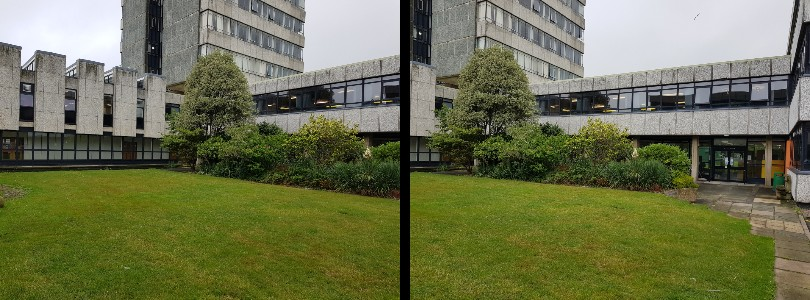
\includegraphics[width=\textwidth]{dataset_pair_provided.jpg}
    \caption{provided（校园建筑）}
\end{subfigure}
\hfill
\begin{subfigure}[b]{0.48\textwidth}
    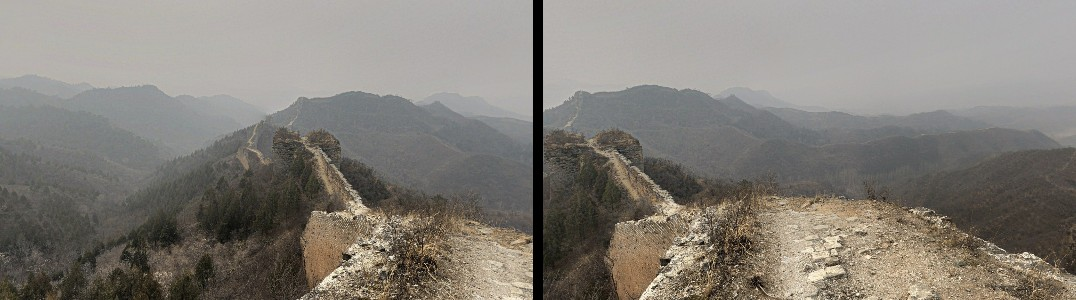
\includegraphics[width=\textwidth]{dataset_pair_GreatWall.jpg}
    \caption{GreatWall（长城）}
\end{subfigure}

\vspace{0.5em}
\begin{subfigure}[b]{0.48\textwidth}
    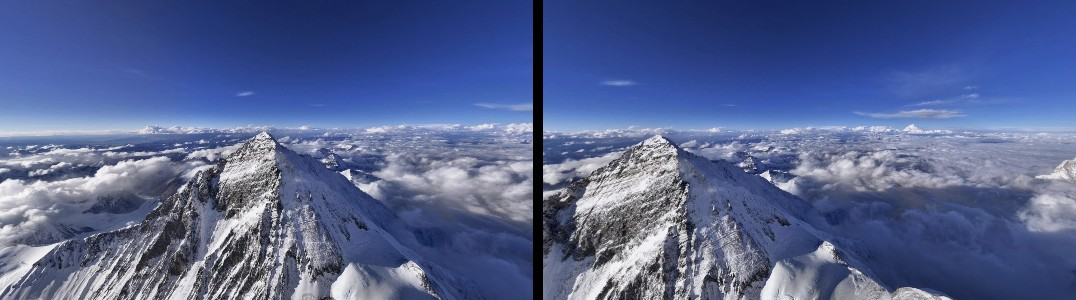
\includegraphics[width=\textwidth]{dataset_pair_Everest.jpg}
    \caption{Everest（珠穆朗玛峰）}
\end{subfigure}
\hfill
\begin{subfigure}[b]{0.48\textwidth}
    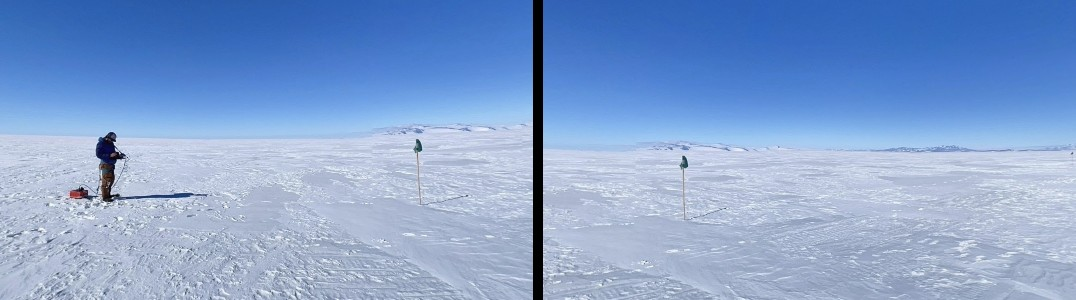
\includegraphics[width=\textwidth]{dataset_pair_Antarctica.jpg}
    \caption{Antarctica（南极洲）}
\end{subfigure}

\vspace{0.5em}
\begin{subfigure}[b]{0.48\textwidth}
    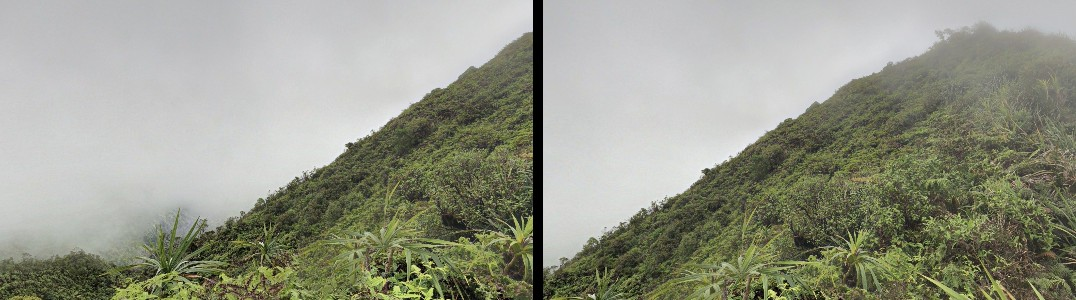
\includegraphics[width=\textwidth]{dataset_pair_Honolulu.jpg}
    \caption{Honolulu（热带山坡）}
\end{subfigure}
\caption{拼接效果优秀的五对图像数据集（左图-右图并排展示）}
\label{fig:dataset_good}
\end{figure}

\begin{figure}[H]
\centering
\begin{subfigure}[b]{0.48\textwidth}
    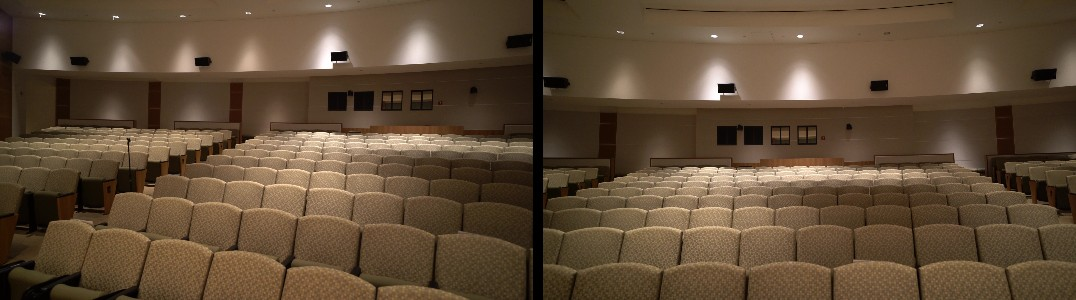
\includegraphics[width=\textwidth]{dataset_pair_Auditorium.jpg}
    \caption{Auditorium（礼堂，相机平移）}
\end{subfigure}
\hfill
\begin{subfigure}[b]{0.48\textwidth}
    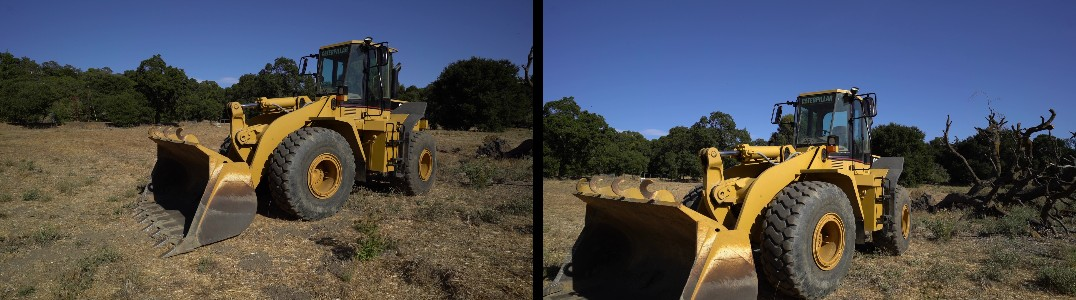
\includegraphics[width=\textwidth]{dataset_pair_Caterpillar.jpg}
    \caption{Caterpillar（推土机，深度变化）}
\end{subfigure}

\vspace{0.5em}
\begin{subfigure}[b]{0.48\textwidth}
    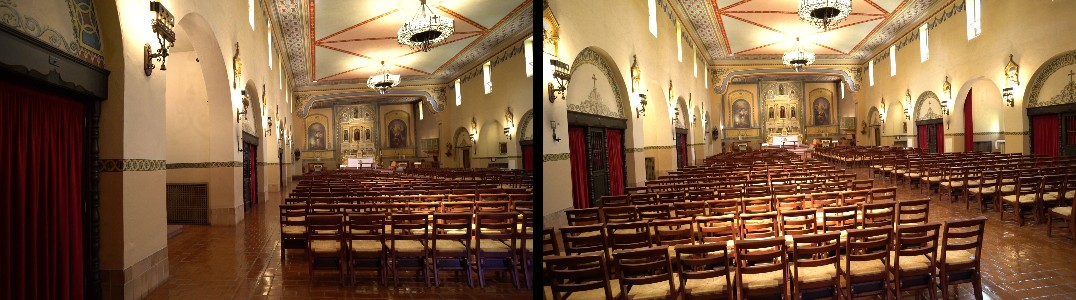
\includegraphics[width=\textwidth]{dataset_pair_Church.jpg}
    \caption{Church（教堂，室内视差）}
\end{subfigure}
\hfill
\begin{subfigure}[b]{0.48\textwidth}
    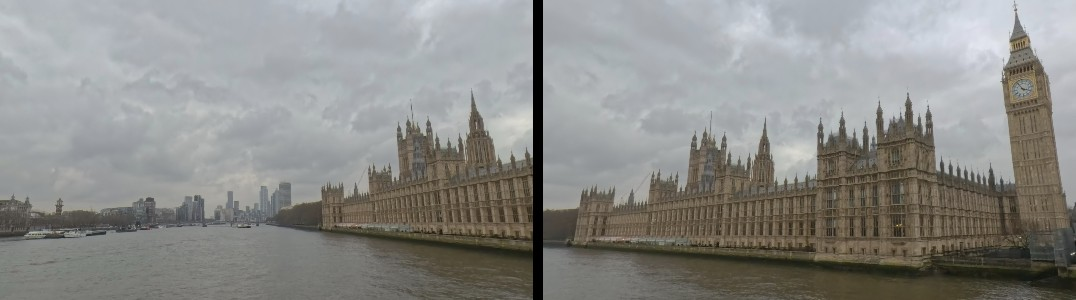
\includegraphics[width=\textwidth]{dataset_pair_BigBen.jpg}
    \caption{BigBen（大本钟，大视角变化）}
\end{subfigure}
\caption{困难场景数据集（存在相机平移、深度变化或大视角旋转）}
\label{fig:dataset_hard}
\end{figure}

\subsection{数据集设计考虑}

以上数据集中，拼接效果为\textbf{优}的五对数据均保证图像对之间均保持至少70\%的重叠区域，且两张图像间只有相机旋转，以满足作业要求。但是数据集在设计上也有意涵盖了不同的场景类型和难度等级。除了使用Google Earth街景截取的，只有旋转操作因而较好地满足了单应性变换的假设条件的数据以外，我们也引入了来自Tanks and Temples数据集的三组图像，他们的相机存在明显的平移运动，且场景具有显著的深度变化，违反了单应性模型的平面场景或纯旋转假设，导致拼接产生伪影。我们希望以此说明算法的局限与边界。而Big Ben数据因为视角变化较大，拼接后会有较大的镜头畸变。所有这些困难场景都被我们有意保留在数据集中，用于后续分析算法的适用范围和局限性。

% ============================================================
\section{特征检测}

本节实现并比较了Harris角点检测和SIFT特征点检测两种方法。

\subsection{Harris角点检测}

\subsubsection{算法原理}

Harris角点检测器通过分析图像灰度在各方向上的变化来识别角点。对于图像窗口内的每个像素，计算结构张量（Structure Tensor）：
\begin{equation}
M = \sum_{(x,y) \in W} w(x,y) \begin{bmatrix} I_x^2 & I_xI_y \\ I_xI_y & I_y^2 \end{bmatrix}
\end{equation}
其中$I_x$、$I_y$为图像梯度，$w(x,y)$为高斯加权函数。

角点响应函数定义为：
\begin{equation}
R = \det(M) - k \cdot \text{trace}(M)^2
\end{equation}
当$R$大于阈值时，该点被判定为角点。

\subsubsection{实现细节}

本实现中Harris检测器的参数选取如下：邻域大小 $\text{block\_size} = 2$，Sobel算子孔径 $\text{ksize} = 3$，Harris自由参数 $k = 0.04$。检测阈值设定为最大响应值的1\%。为减少冗余检测结果，进一步采用$5\times5$矩形核的形态学膨胀操作进行非极大值抑制，仅保留局部极大值点作为最终角点。

\subsection{SIFT特征检测}

\subsubsection{算法原理}

SIFT (Scale-Invariant Feature Transform) 通过以下步骤检测具有尺度和旋转不变性的特征点：

\begin{enumerate}
    \item \textbf{尺度空间构建}：通过不同尺度的高斯模糊构建高斯金字塔，相邻层相减得到DoG (Difference of Gaussians) 金字塔。
    \item \textbf{关键点定位}：在DoG空间中寻找局部极值点，通过二次插值精确定位，并去除低对比度点和边缘响应点。
    \item \textbf{方向分配}：统计关键点邻域的梯度方向直方图，以主方向为特征点的方向。
\end{enumerate}

\subsubsection{实现参数}

本实现调用OpenCV库的SIFT接口，主要参数为：每个octave的层数 $\text{nOctaveLayers} = 3$，对比度阈值 $\text{contrastThreshold} = 0.04$，边缘阈值 $\text{edgeThreshold} = 10$，初始高斯模糊参数 $\sigma = 1.6$。

\subsection{检测结果对比}

\begin{figure}[H]
\centering
\begin{subfigure}[b]{0.48\textwidth}
    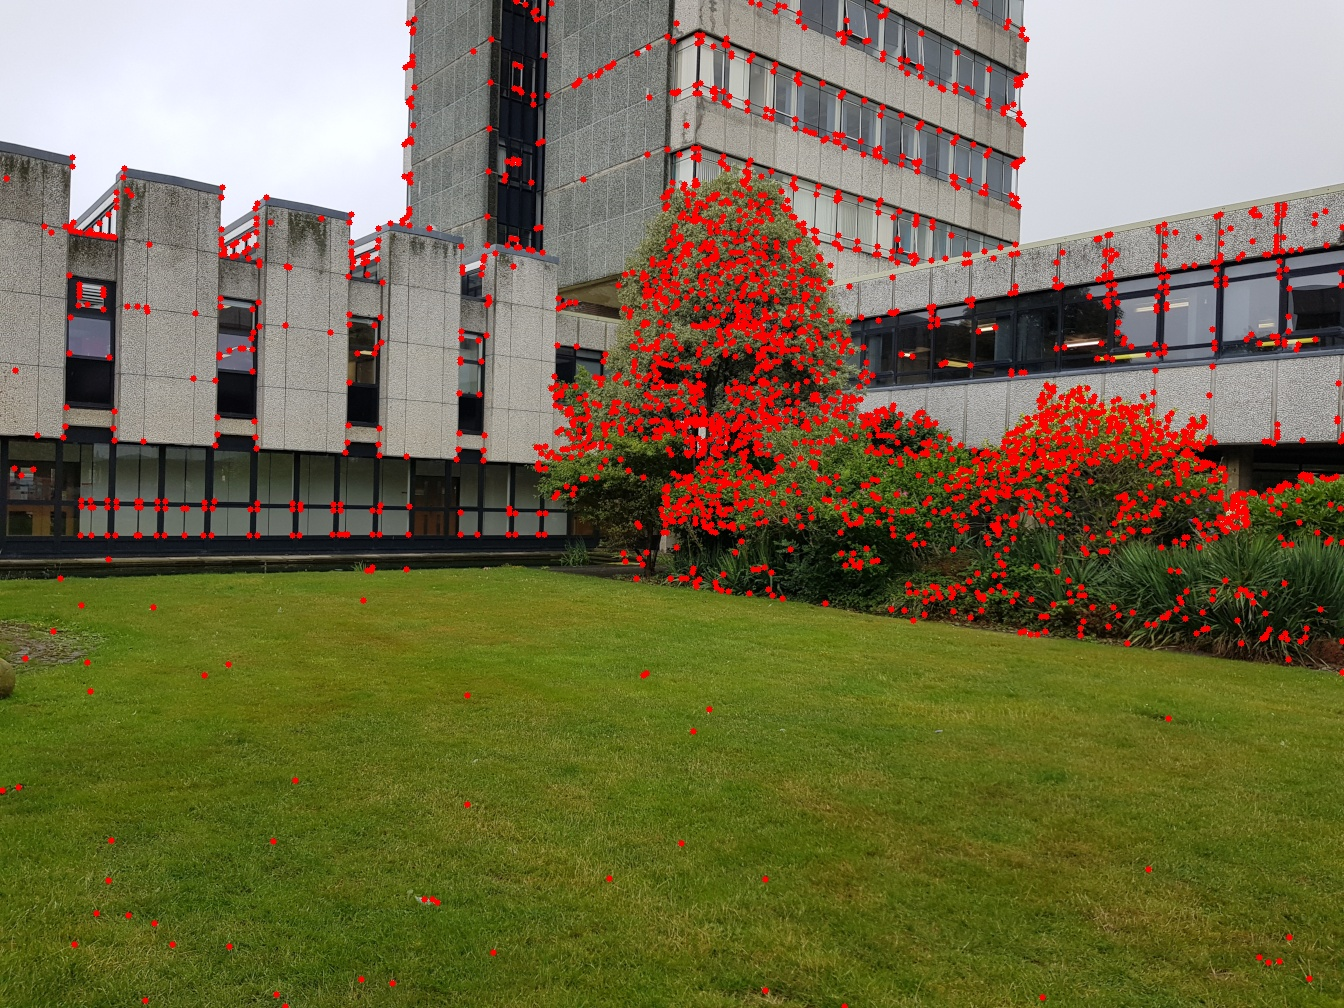
\includegraphics[width=\textwidth]{harris_only_provided.jpg}
    \caption{Harris角点检测结果（红色）}
\end{subfigure}
\hfill
\begin{subfigure}[b]{0.48\textwidth}
    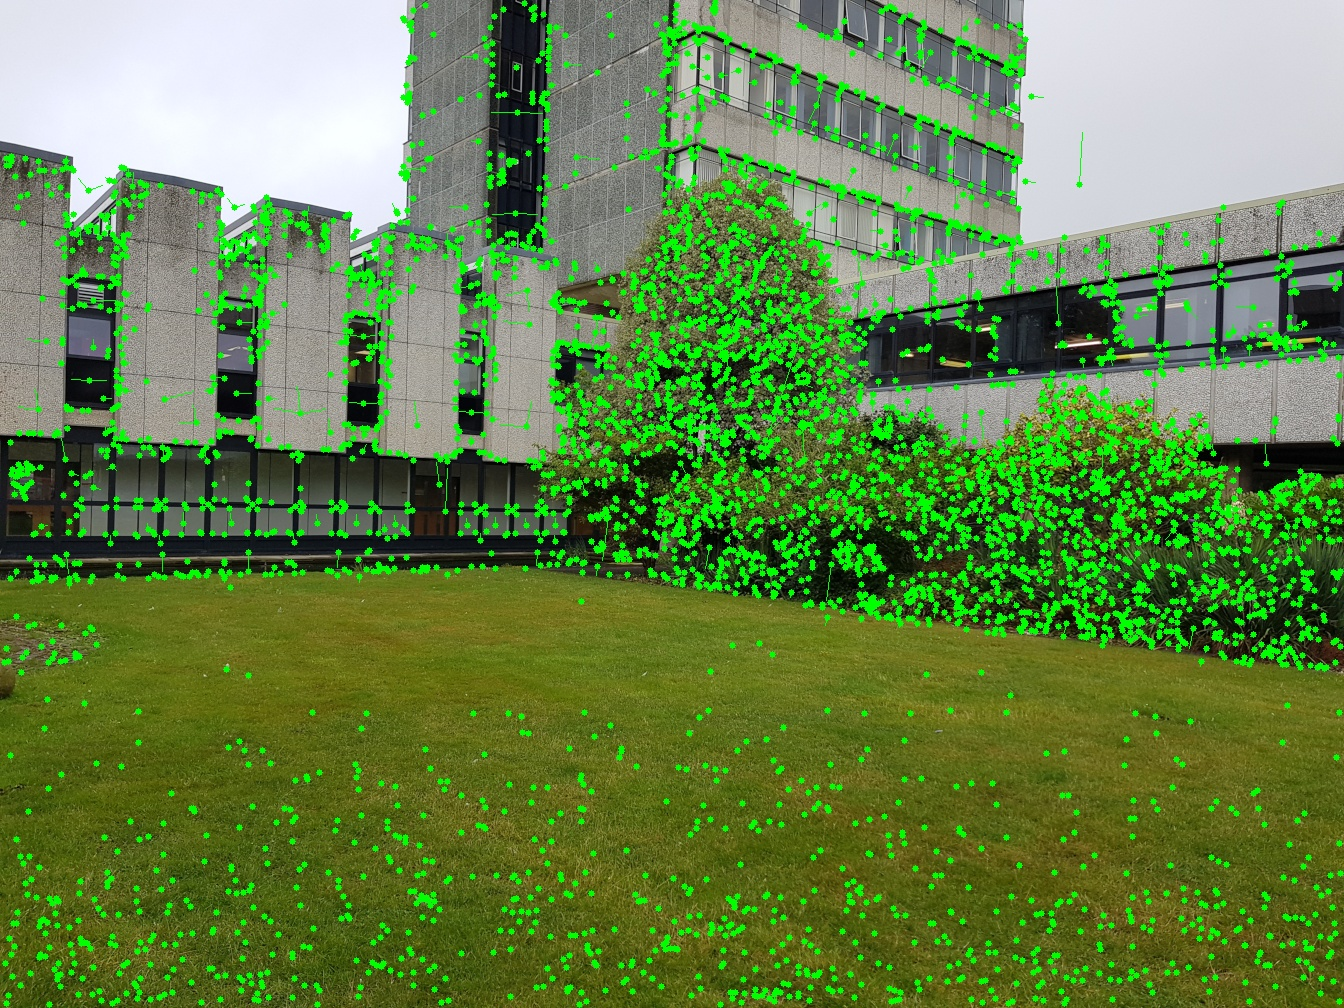
\includegraphics[width=\textwidth]{sift_only_provided.jpg}
    \caption{SIFT特征点检测结果（绿色，含方向）}
\end{subfigure}
\caption{provided图像的特征检测对比}
\label{fig:detection_provided}
\end{figure}

\begin{figure}[H]
\centering
\begin{subfigure}[b]{0.48\textwidth}
    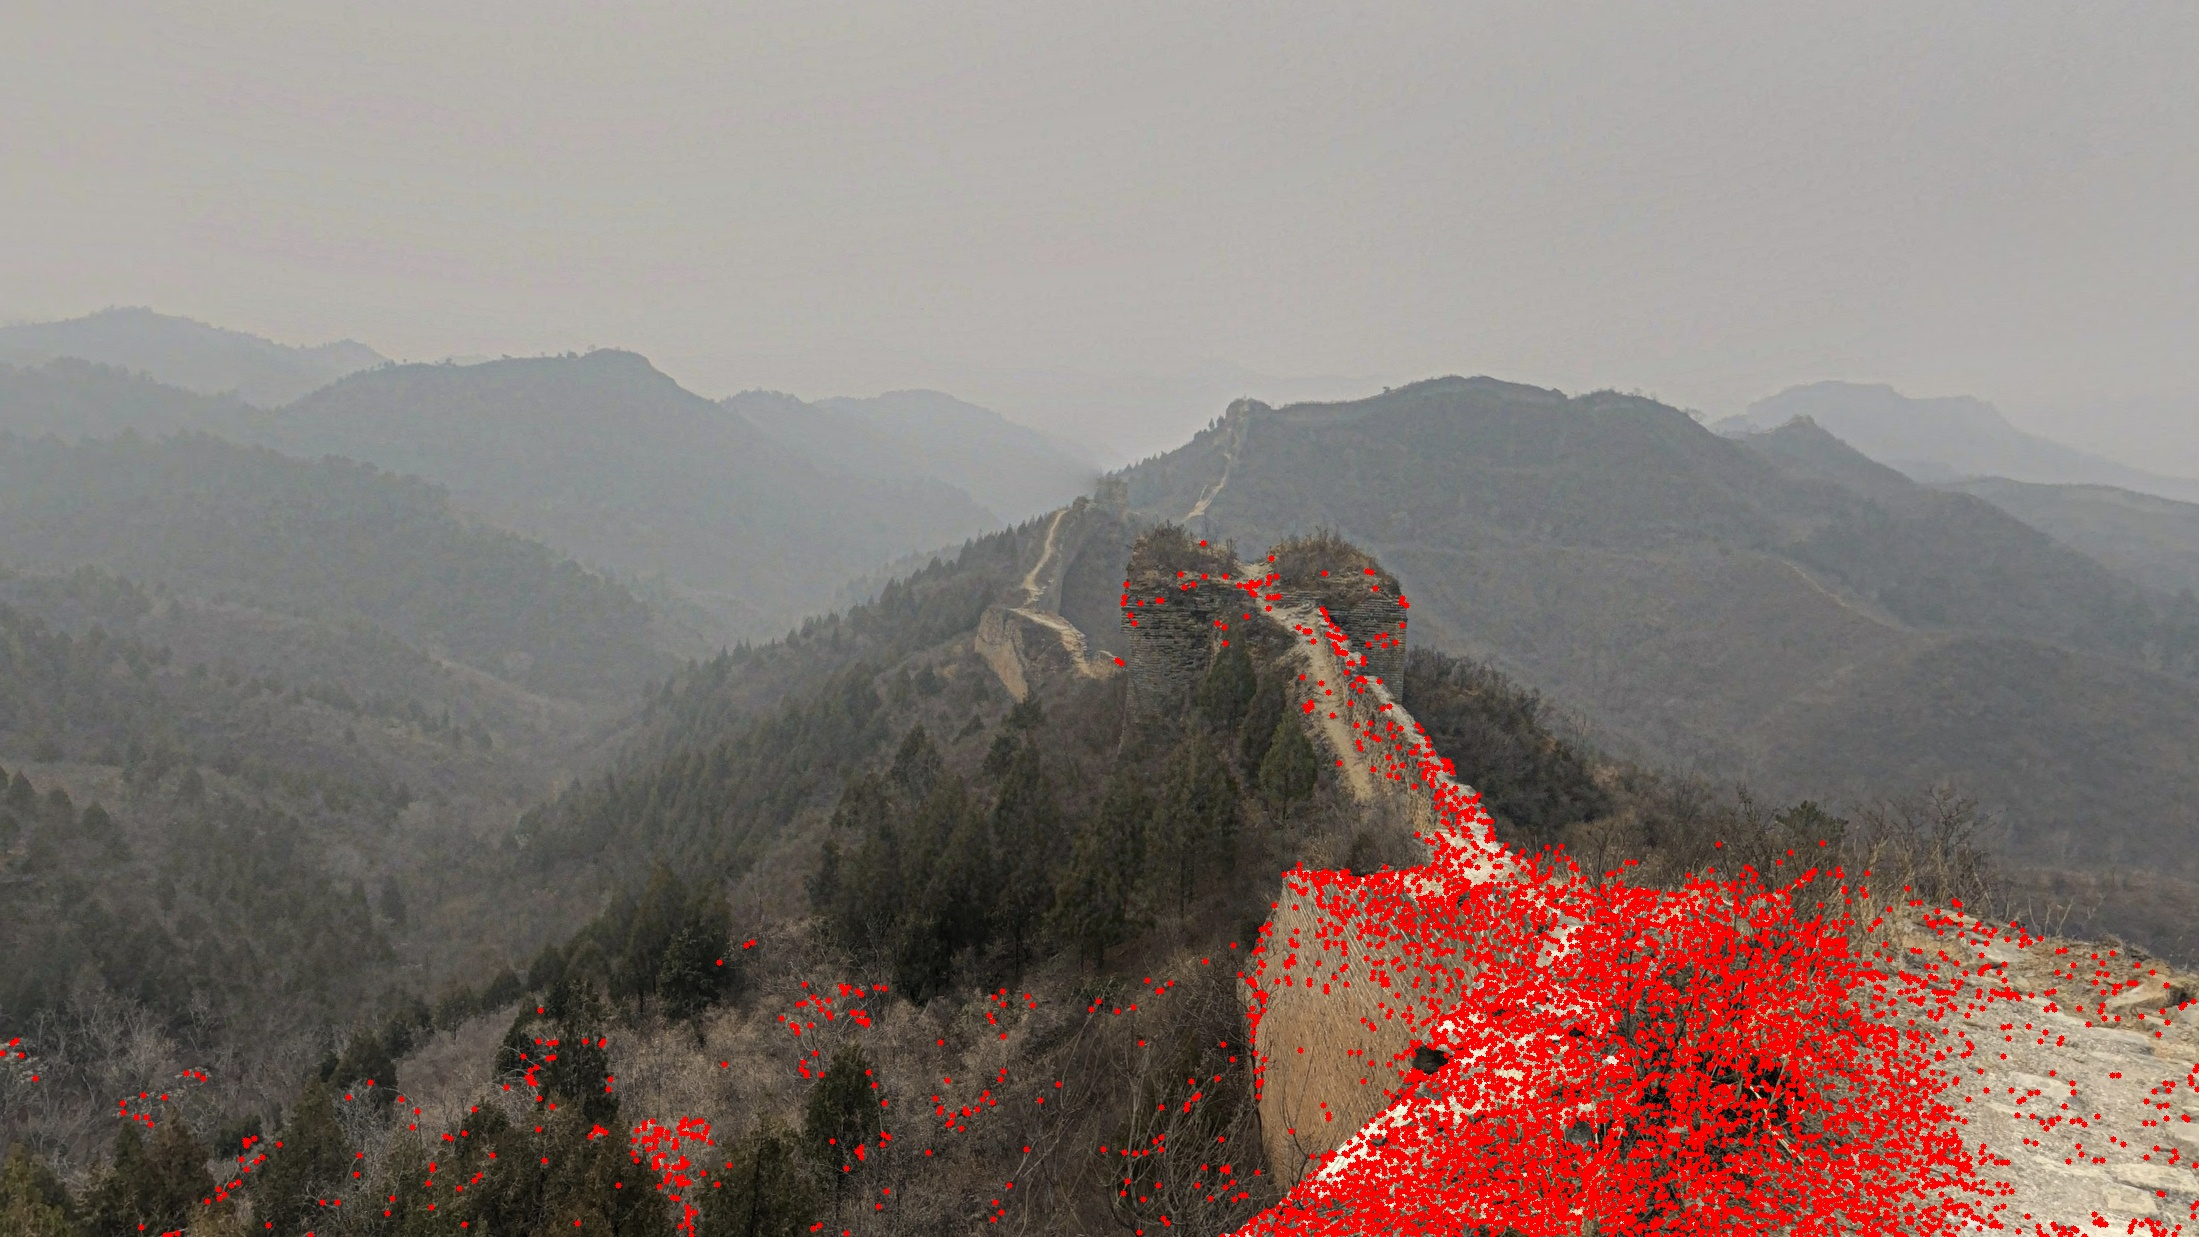
\includegraphics[width=\textwidth]{harris_only_GreatWall.jpg}
    \caption{Harris角点检测结果}
\end{subfigure}
\hfill
\begin{subfigure}[b]{0.48\textwidth}
    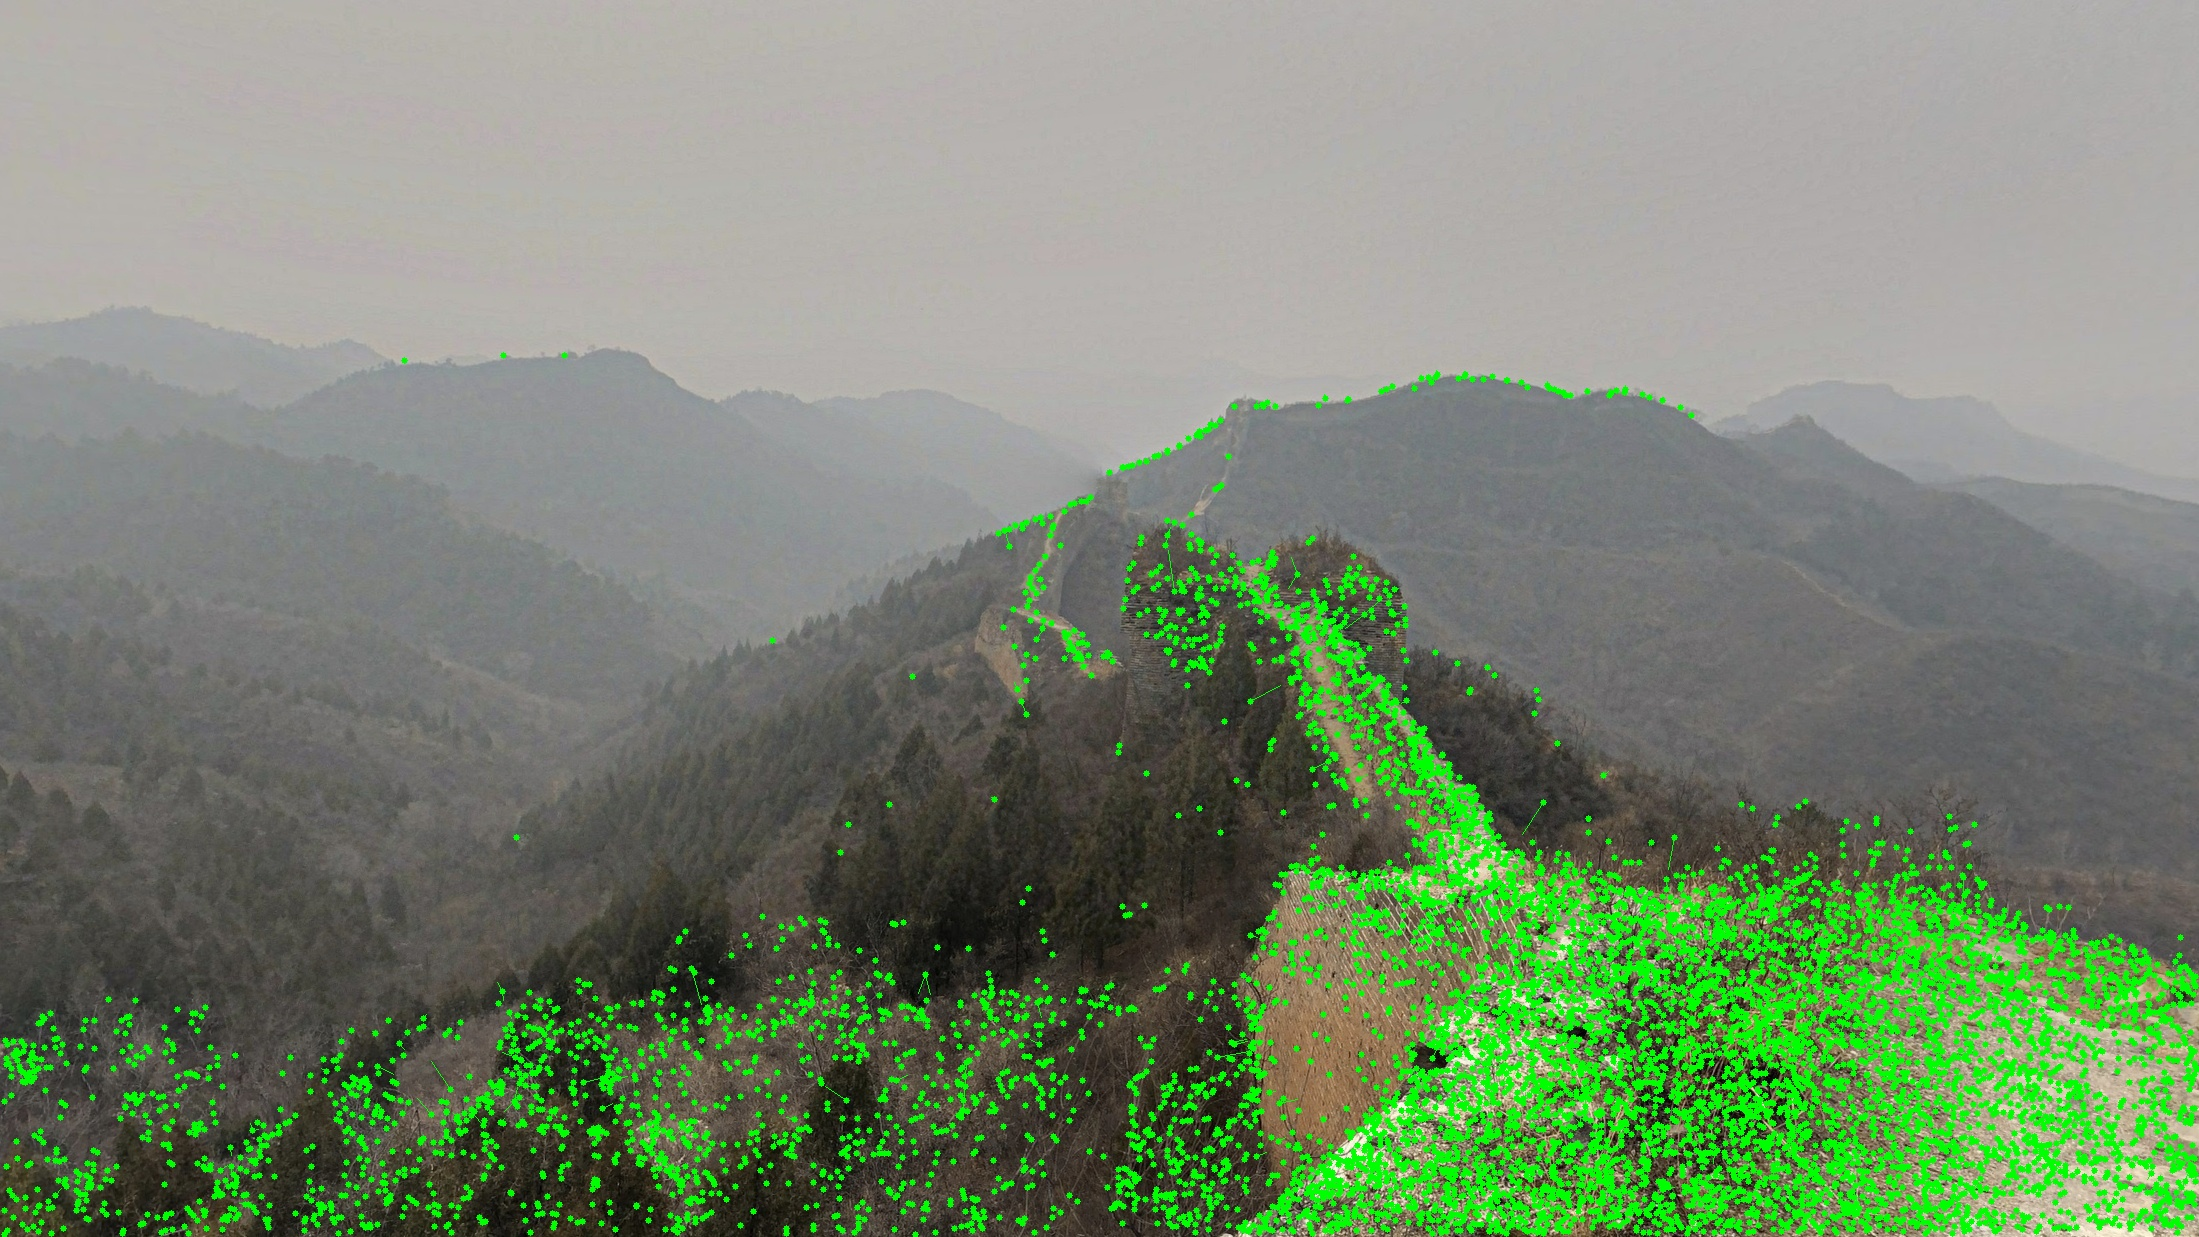
\includegraphics[width=\textwidth]{sift_only_GreatWall.jpg}
    \caption{SIFT特征点检测结果}
\end{subfigure}
\caption{GreatWall图像的特征检测对比}
\label{fig:detection_greatwall}
\end{figure}

\begin{table}[H]
\centering
\caption{Harris与SIFT特征检测数量对比}
\label{tab:detection_comparison}
\begin{tabular}{lrrrr}
\toprule
\textbf{图像对} & \textbf{Harris(左)} & \textbf{Harris(右)} & \textbf{SIFT(左)} & \textbf{SIFT(右)} \\
\midrule
provided & 2595 & 4475 & 6841 & 7273 \\
Auditorium & 217 & 143 & 4574 & 4197 \\
Caterpillar & 2843 & 2399 & 11933 & 8711 \\
Church & 1698 & 3251 & 7312 & 11577 \\
GreatWall & 5337 & 10212 & 9962 & 14362 \\
BigBen & 950 & 350 & 1959 & 4002 \\
Antarctica & 1183 & 595 & 6952 & 2281 \\
Honolulu & 8818 & 7934 & 19529 & 23816 \\
Everest & 5505 & 4079 & 11638 & 10564 \\
\bottomrule
\end{tabular}
\end{table}

\subsection{对比分析}

表\ref{tab:detection_comparison}的数据以及图\ref{fig:detection_provided}和图\ref{fig:detection_greatwall}的可视化结果揭示了两种检测方法之间的显著差异。

在检测数量方面，SIFT通常检测到远多于Harris的特征点。以Auditorium场景为例，Harris仅检测到143个角点，而SIFT检测到4197个关键点，差异超过一个数量级。这一差距的根源在于Harris仅对图像中的角点结构产生响应，而SIFT在多尺度DoG空间中能够捕获包括斑块、纹理变化在内的多种显著结构。

在空间分布方面，Harris角点倾向于集中在纹理丰富的边缘区域，例如建筑物的轮廓线和窗户边角。相比之下，SIFT关键点在图像中的分布更为均匀，覆盖了纹理区域、渐变区域和斑块区域。这种均匀分布对后续的特征匹配和单应性估计具有重要意义，因为空间分布良好的匹配点有助于提高变换矩阵估计的数值稳定性。

两种方法最本质的区别在于特征信息的丰富程度。Harris检测的角点仅包含位置信息，缺乏尺度和方向属性；而SIFT关键点同时携带了精确的尺度参数和主方向信息，这为后续构建具有旋转和尺度不变性的描述子奠定了基础。


% ============================================================
\section{特征描述}

在检测到兴趣点后，需要为每个特征点构建描述子，作为后续匹配的依据。本文实现了两种描述子：SIFT（高精度浮点描述子）和ORB（低成本二进制描述子）。

\subsection{SIFT描述子}

\subsubsection{算法原理}

SIFT描述子以关键点为中心，在其主方向对齐的坐标系中构建：
\begin{enumerate}
    \item 取关键点周围$16\times16$像素的邻域。
    \item 将邻域划分为$4\times4$个子区域（每个子区域$4\times4$像素）。
    \item 在每个子区域内统计8个方向的梯度直方图。
    \item 拼接所有子区域的直方图得到$4\times4\times8 = 128$维向量。
    \item 对向量进行L2归一化，截断大于0.2的分量后再次归一化。
\end{enumerate}

SIFT描述子的维度为128，每个分量为浮点数（float32），因此每个描述子占用$128\times4 = 512$字节。其自然匹配度量为L2距离（SSD）。

\subsection{ORB描述子（低成本二进制描述子）}

\subsubsection{算法原理}

ORB (Oriented FAST and Rotated BRIEF) 是一种高效的二进制描述子：
\begin{enumerate}
    \item 使用FAST检测关键点，并通过图像矩 (image moments) 计算关键点方向。
    \item 以关键点方向旋转BRIEF采样模式（steered BRIEF），实现旋转不变性。
    \item 对旋转后的采样点对进行灰度比较，生成256位（32字节）的二进制描述子。
\end{enumerate}

与SIFT相比，ORB在存储效率上具有显著优势：每个描述子仅占32字节，而SIFT为512字节，压缩比达到$16\times$。在计算速度方面，ORB的检测与描述阶段通常比SIFT快7--8倍。在匹配度量上，ORB使用Hamming距离进行描述子比较，仅需执行异或（XOR）和比特计数（popcount）操作，计算效率远高于SIFT所需的浮点L2距离计算。

\subsection{距离度量}

两种描述子对应不同的距离度量方式。对于SIFT的128维浮点描述子，自然的距离度量为平方差和（SSD）：
\begin{equation}
d(X, Y) = \|X - Y\|^2 = \sum_{i=1}^{128}(x_i - y_i)^2
\end{equation}

对于ORB的256位二进制描述子，则使用Hamming距离：
\begin{equation}
d_H(X, Y) = \text{popcount}(X \oplus Y)
\end{equation}
即将两个二进制串进行异或运算后统计结果中1的个数，反映了两个描述子在多少个比特位上存在差异。

% ============================================================
\section{特征匹配}

特征匹配的目标是：对于图像1中的每个特征，在图像2中找到最佳匹配。本节实现了两种距离度量策略，并对两种描述子进行了全面对比。

\subsection{距离度量方法}

\subsubsection{SSD最近邻匹配}

对于图像1中的每个描述子$X_i$，计算它与图像2中所有描述子的SSD距离，取距离最小者为匹配结果：
\begin{equation}
\text{match}(X_i) = \arg\min_{Y_j} \|X_i - Y_j\|^2
\end{equation}

实现中使用了向量化计算加速：利用展开式$\|a-b\|^2 = \|a\|^2 + \|b\|^2 - 2a^Tb$，将距离矩阵的计算转化为矩阵乘法，避免了$O(N \times M)$的逐对循环。

\subsubsection{比值检验（Ratio Test）}

Lowe提出的比值检验通过比较最近匹配与次近匹配的距离来过滤歧义匹配：
\begin{equation}
\text{ratio} = \frac{d_{\text{1st}}}{d_{\text{2nd}}}
\end{equation}

当ratio $< 0.7$时，认为该匹配可靠（最近匹配远优于次近匹配，说明匹配具有明确性）。不满足条件的匹配被丢弃。

比值检验的核心思想是：如果一个特征在另一幅图中有多个相似的候选匹配（即$d_{\text{1st}} \approx d_{\text{2nd}}$），则该匹配很可能是错误的。

\subsection{实验一：SSD vs Ratio Test（SIFT描述子）}

\begin{table}[H]
\centering
\caption{SSD最近邻 vs Ratio Test 匹配准确率对比（SIFT描述子）}
\label{tab:ssd_vs_rt}
\begin{tabular}{lrrrrrr}
\toprule
& \multicolumn{3}{c}{\textbf{SSD最近邻}} & \multicolumn{3}{c}{\textbf{Ratio Test}} \\
\cmidrule(lr){2-4} \cmidrule(lr){5-7}
\textbf{图像对} & 匹配数 & 内点数 & 准确率 & 匹配数 & 内点数 & 准确率 \\
\midrule
provided & 6841 & 1966 & 28.74\% & 2299 & 1786 & 77.69\% \\
Auditorium & 4574 & 782 & 17.10\% & 1208 & 543 & 44.95\% \\
Caterpillar & 11933 & 118 & 0.99\% & 1120 & 296 & 26.43\% \\
Church & 7312 & 245 & 3.35\% & 1542 & 395 & 25.62\% \\
GreatWall & 9962 & 3498 & 35.12\% & 3437 & 3345 & 97.32\% \\
BigBen & 1959 & 886 & 45.23\% & 913 & 825 & 90.36\% \\
Antarctica & 6952 & 765 & 11.00\% & 957 & 745 & 77.85\% \\
Honolulu & 19529 & 6669 & 34.14\% & 6663 & 6416 & 96.29\% \\
Everest & 11638 & 3416 & 29.35\% & 3432 & 3113 & 90.71\% \\
\midrule
\textbf{平均} & & & \textbf{23.0\%} & & & \textbf{69.6\%} \\
\bottomrule
\end{tabular}
\end{table}

\begin{figure}[H]
\centering
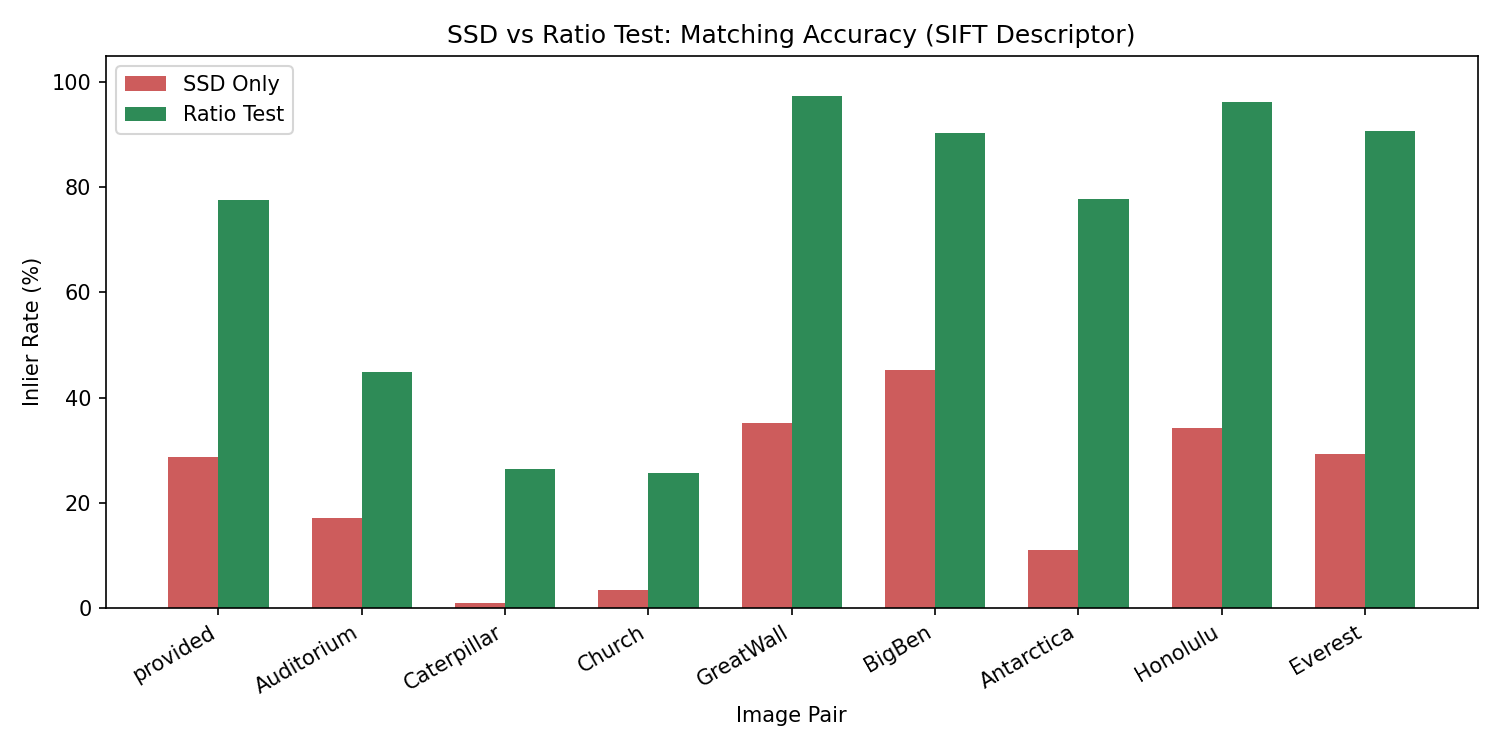
\includegraphics[width=0.85\textwidth]{chart_ssd_vs_rt_accuracy.png}
\caption{SSD vs Ratio Test 匹配准确率对比}
\label{fig:ssd_vs_rt}
\end{figure}

\subsubsection{分析}

表\ref{tab:ssd_vs_rt}和图\ref{fig:ssd_vs_rt}的实验结果清楚地展示了Ratio Test的优势。在全部9对图像上，Ratio Test将平均匹配准确率从23.0\%大幅提升至69.6\%，提升约3倍。这一结果表明，SSD最近邻匹配中存在大量歧义匹配——即一个特征在目标图像中存在多个距离相近的候选，而Ratio Test通过其比值过滤机制有效地识别并剔除了这些不可靠的对应关系。

另一方面，Ratio Test在大幅减少匹配总数的同时，对正确匹配的保留率极高。以provided图像对为例，匹配数从6841降至2299（减少66\%），但RANSAC内点数仅从1966降至1786（保留了91\%的正确匹配），说明被过滤掉的绝大多数是错误匹配。

实验还揭示了匹配准确率对场景特性的强烈依赖。在纹理丰富且具有多样性的场景中（如GreatWall准确率达97.32\%，Everest达90.71\%），特征的区分度高，即使是SSD最近邻也能获得约30\%的准确率，而Ratio Test则能进一步将其提升至90\%以上。然而，在以重复纹理为主的场景中（如Caterpillar仅24.98\%，Church仅25.62\%），大量相似特征导致匹配歧义难以消除，Ratio Test的准确率同样受限。

\subsection{实验二：SIFT vs ORB描述子对比}

\begin{table}[H]
\centering
\caption{SIFT vs ORB 描述子匹配性能对比}
\label{tab:sift_vs_orb}
\begin{tabular}{lrrrrrr}
\toprule
& \multicolumn{3}{c}{\textbf{SIFT}} & \multicolumn{3}{c}{\textbf{ORB}} \\
\cmidrule(lr){2-4} \cmidrule(lr){5-7}
\textbf{图像对} & 匹配数 & 准确率 & 耗时(s) & 匹配数 & 准确率 & 耗时(s) \\
\midrule
provided & 2299 & 77.69\% & 0.84 & 1274 & 93.33\% & 2.15 \\
Auditorium & 1208 & 44.95\% & 0.55 & 826 & 72.52\% & 2.13 \\
Caterpillar & 1120 & 26.43\% & 1.57 & 330 & 40.00\% & 2.20 \\
Church & 1542 & 25.62\% & 1.42 & 177 & 33.33\% & 2.15 \\
GreatWall & 3437 & 97.32\% & 2.36 & 1364 & 98.75\% & 2.20 \\
BigBen & 913 & 90.36\% & 0.59 & 810 & 91.60\% & 2.11 \\
Antarctica & 957 & 77.85\% & 0.69 & 198 & 91.92\% & 2.01 \\
Honolulu & 6663 & 96.29\% & 6.11 & 761 & 97.77\% & 2.19 \\
Everest & 3432 & 90.71\% & 2.15 & 747 & 97.86\% & 2.18 \\
\midrule
\textbf{平均} & & \textbf{69.62\%} & \textbf{1.81} & & \textbf{78.50\%} & \textbf{2.15} \\
\bottomrule
\end{tabular}
\end{table}

\begin{figure}[H]
\centering
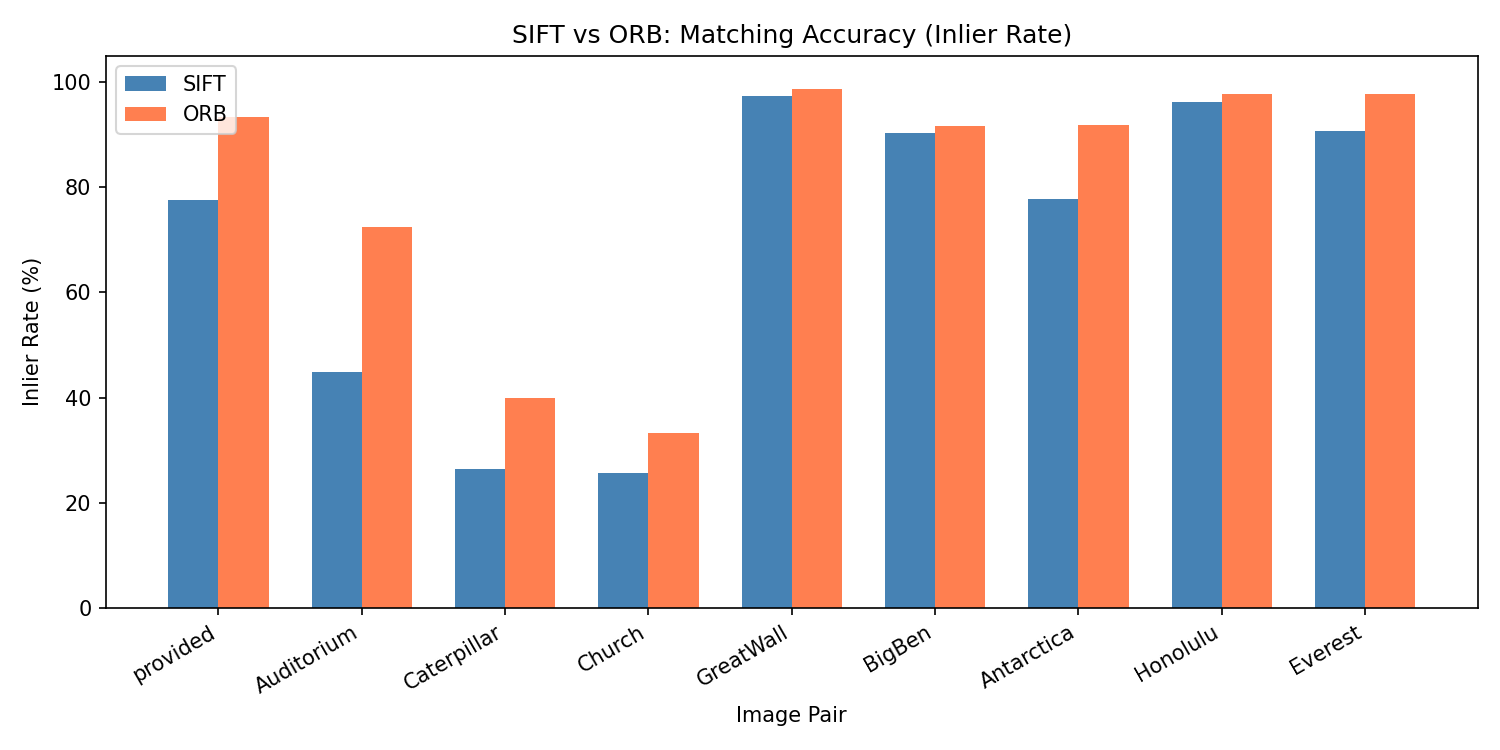
\includegraphics[width=0.85\textwidth]{chart_sift_vs_orb_accuracy.png}
\caption{SIFT vs ORB 匹配准确率对比}
\label{fig:sift_vs_orb_acc}
\end{figure}

\begin{figure}[H]
\centering
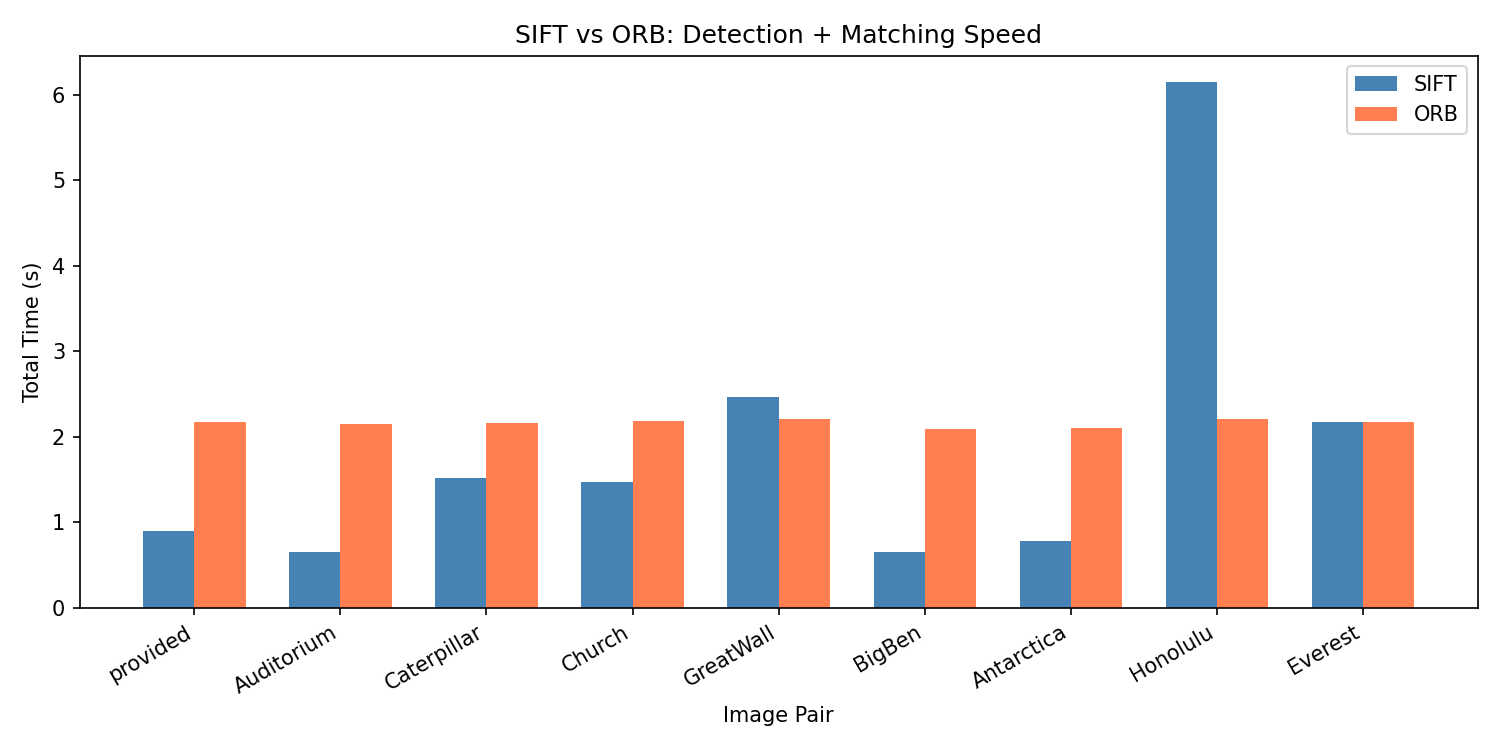
\includegraphics[width=0.85\textwidth]{chart_sift_vs_orb_speed.png}
\caption{SIFT vs ORB 检测+匹配总耗时对比}
\label{fig:sift_vs_orb_speed}
\end{figure}

\subsubsection{分析}

表\ref{tab:sift_vs_orb}以及图\ref{fig:sift_vs_orb_acc}、图\ref{fig:sift_vs_orb_speed}的结果揭示了两种描述子之间的多维度权衡。

在准确率方面，ORB的平均内点率（78.50\%）略高于SIFT（69.62\%）。然而，这一数值差异并不意味着ORB的描述能力优于SIFT。仔细观察可以发现，ORB的特征点数量被限制为5000个（通过nfeatures参数控制），而SIFT没有施加此限制，在Honolulu等纹理密集场景中检测到了多达23816个关键点。更多的特征点意味着更大的搜索空间和更高的歧义概率，这在一定程度上拉低了SIFT的内点率。

在匹配数量方面，SIFT的优势十分明显。以Honolulu为例，SIFT产生了6663个有效匹配，而ORB仅有761个；在Church场景中，差距更为悬殊——SIFT有1542个匹配，ORB仅177个。对于需要大量高质量对应点的下游任务（如高精度单应性估计、三维重建等），SIFT提供的高召回率具有不可替代的价值。

在速度方面，ORB的特征检测与描述阶段极为高效（约0.04--0.05秒），较SIFT（0.2--0.6秒）快7--8倍。然而，本实现中匹配阶段的耗时呈现出不同的趋势：SIFT的SSD距离矩阵通过$\|a-b\|^2 = \|a\|^2 + \|b\|^2 - 2a^Tb$展开后转化为高效的矩阵乘法，而ORB的Hamming距离矩阵计算采用查表法（lookup table popcount），在5000$\times$5000的规模下约需2.1秒。当SIFT特征点数量较少时（如BigBen仅1959个），其总耗时反而低于ORB。

总的来说，SIFT以更高的计算开销换取了更强的特征区分能力和更高的匹配召回率，适用于离线处理和对匹配质量要求严格的应用场景；ORB则以极低的检测成本和紧凑的二进制表示见长，更适合实时视觉系统和资源受限的嵌入式平台。

\subsection{匹配可视化}

\begin{figure}[H]
\centering
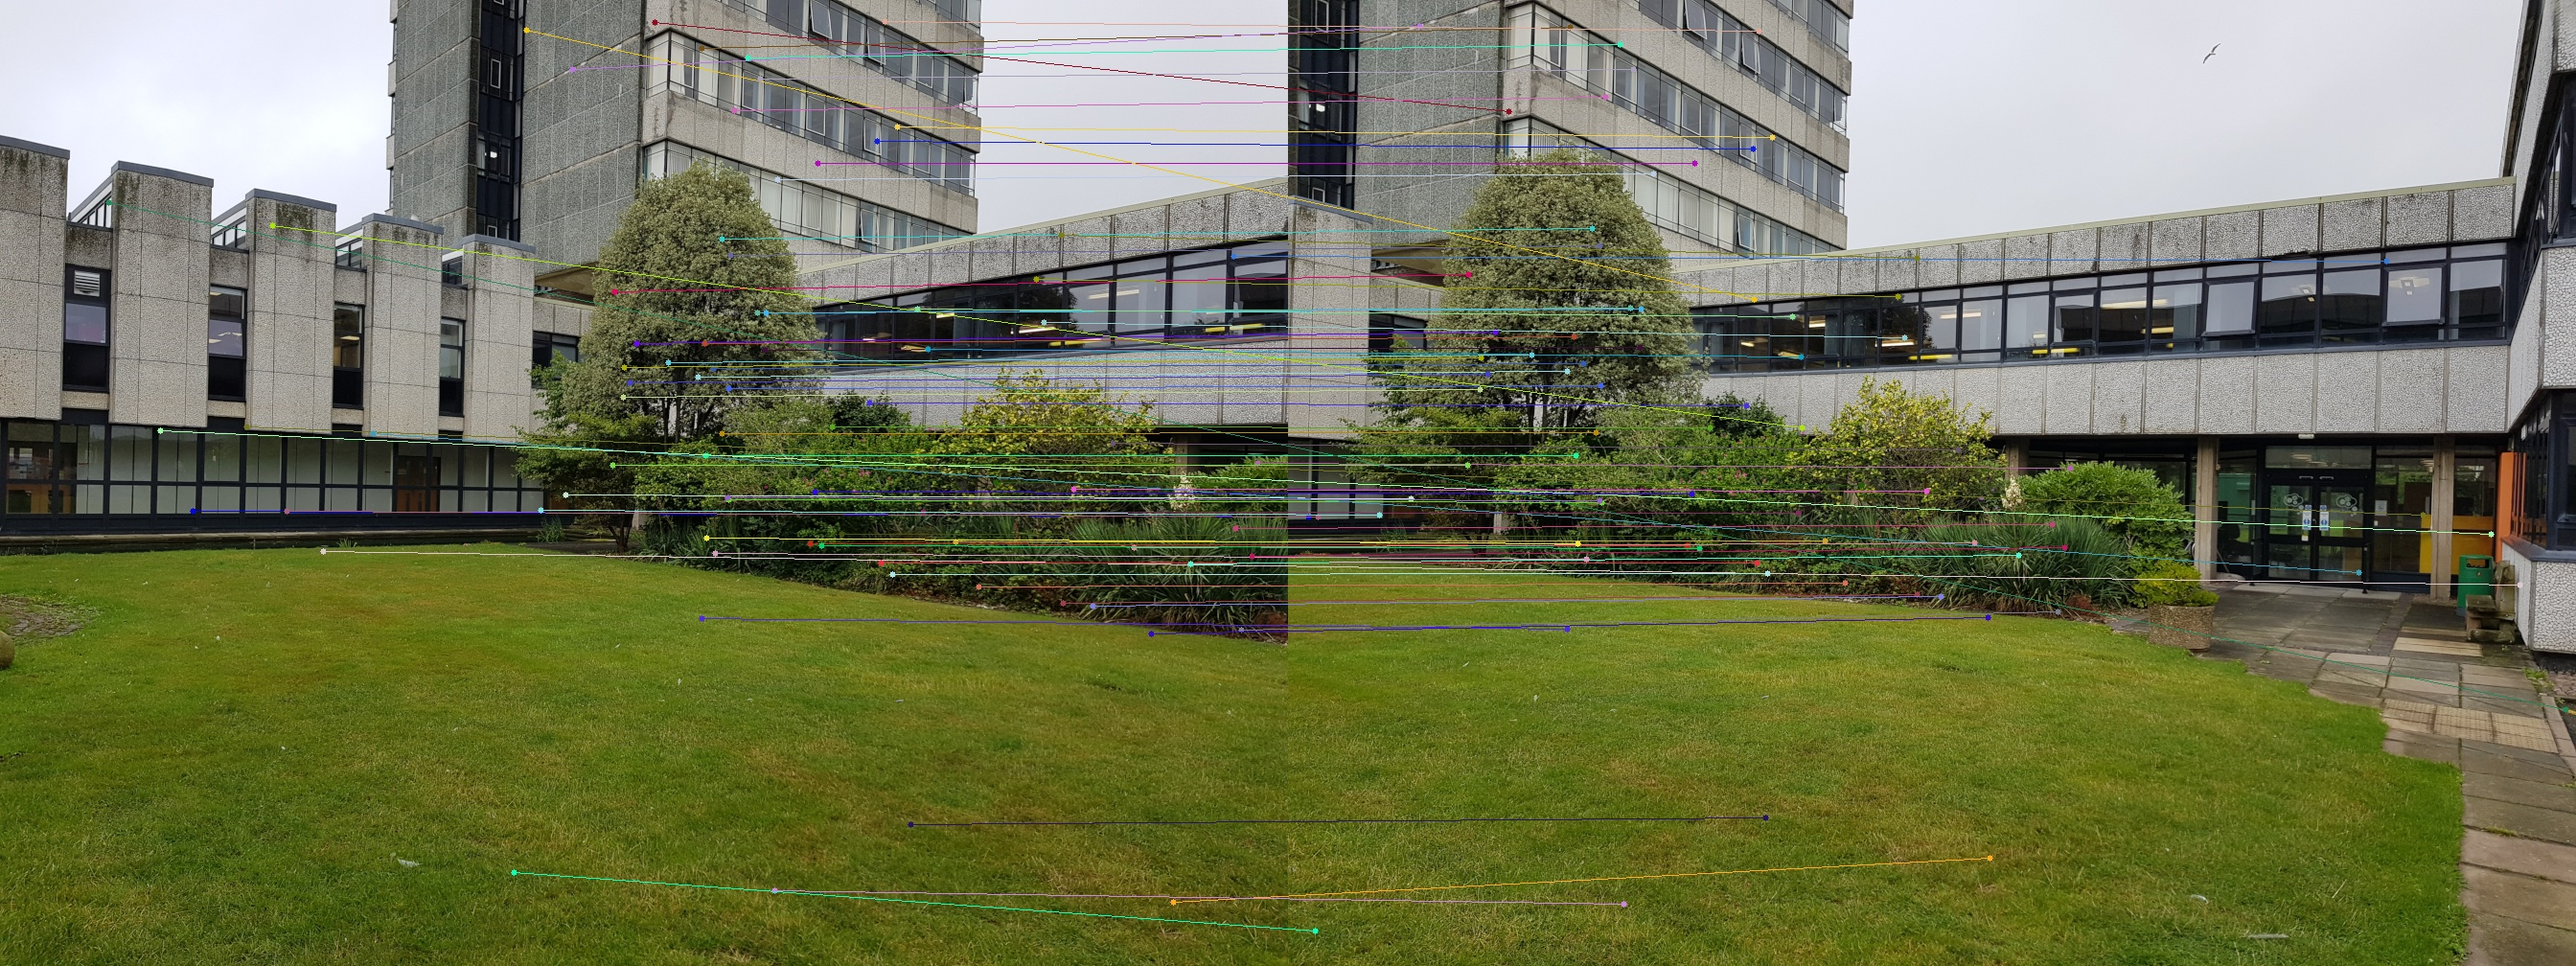
\includegraphics[width=\textwidth]{provided_matches.jpg}
\caption{provided图像对的特征匹配结果（Ratio Test, SIFT描述子）}
\label{fig:match_provided}
\end{figure}

\begin{figure}[H]
\centering
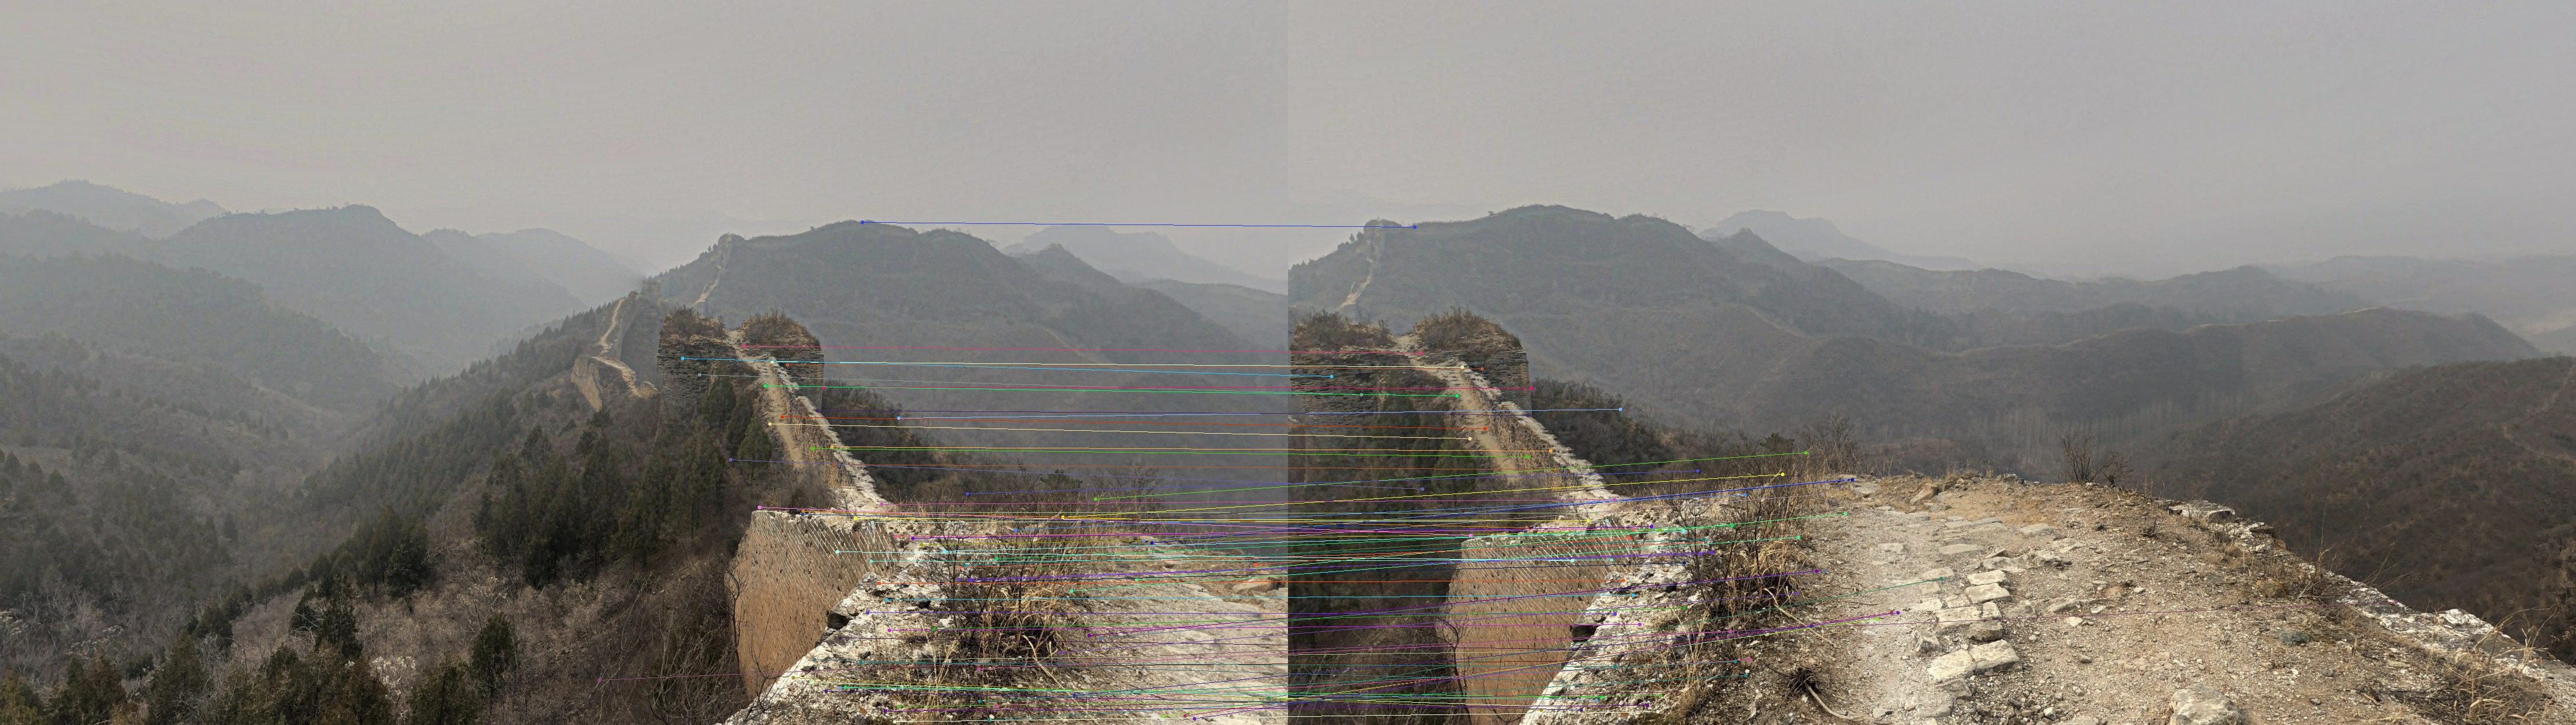
\includegraphics[width=\textwidth]{GreatWall_matches.jpg}
\caption{GreatWall图像对的特征匹配结果}
\label{fig:match_greatwall}
\end{figure}

% ============================================================
\section{图像拼接}

\subsection{单应性矩阵估计}

两幅图像之间的几何关系用$3\times3$单应性矩阵$H$描述，满足：
\begin{equation}
\begin{bmatrix} x' \\ y' \\ 1 \end{bmatrix} \sim H \begin{bmatrix} x \\ y \\ 1 \end{bmatrix}
\end{equation}

使用RANSAC算法鲁棒地估计$H$：
\begin{enumerate}
    \item 随机选取4对匹配点，用DLT (Direct Linear Transform) 计算候选$H$。
    \item 用该$H$对所有匹配点进行重投影，统计重投影误差小于阈值（5像素）的内点数。
    \item 重复迭代，保留内点数最多的$H$。
    \item 用所有内点重新拟合最终的$H$。
\end{enumerate}

本实现使用\texttt{cv2.findHomography}，方法为RANSAC，重投影阈值5.0像素。

\subsection{图像变换与合成}

按照作业要求，拼接流程如下：
\begin{enumerate}
    \item 计算从右图到左图的单应性矩阵$H$。
    \item 使用$H$对右图进行透视变换（warp），输出画布宽度为\textbf{左图宽度 + 右图宽度}。
    \item 将左图内容直接复制到画布的左侧区域$[0:h_1, 0:w_1]$。
\end{enumerate}

重叠区域采用简单覆盖策略：左图像素直接覆盖warp后的右图像素。

\subsection{拼接结果}

\subsubsection{成功案例}

\begin{figure}[H]
\centering
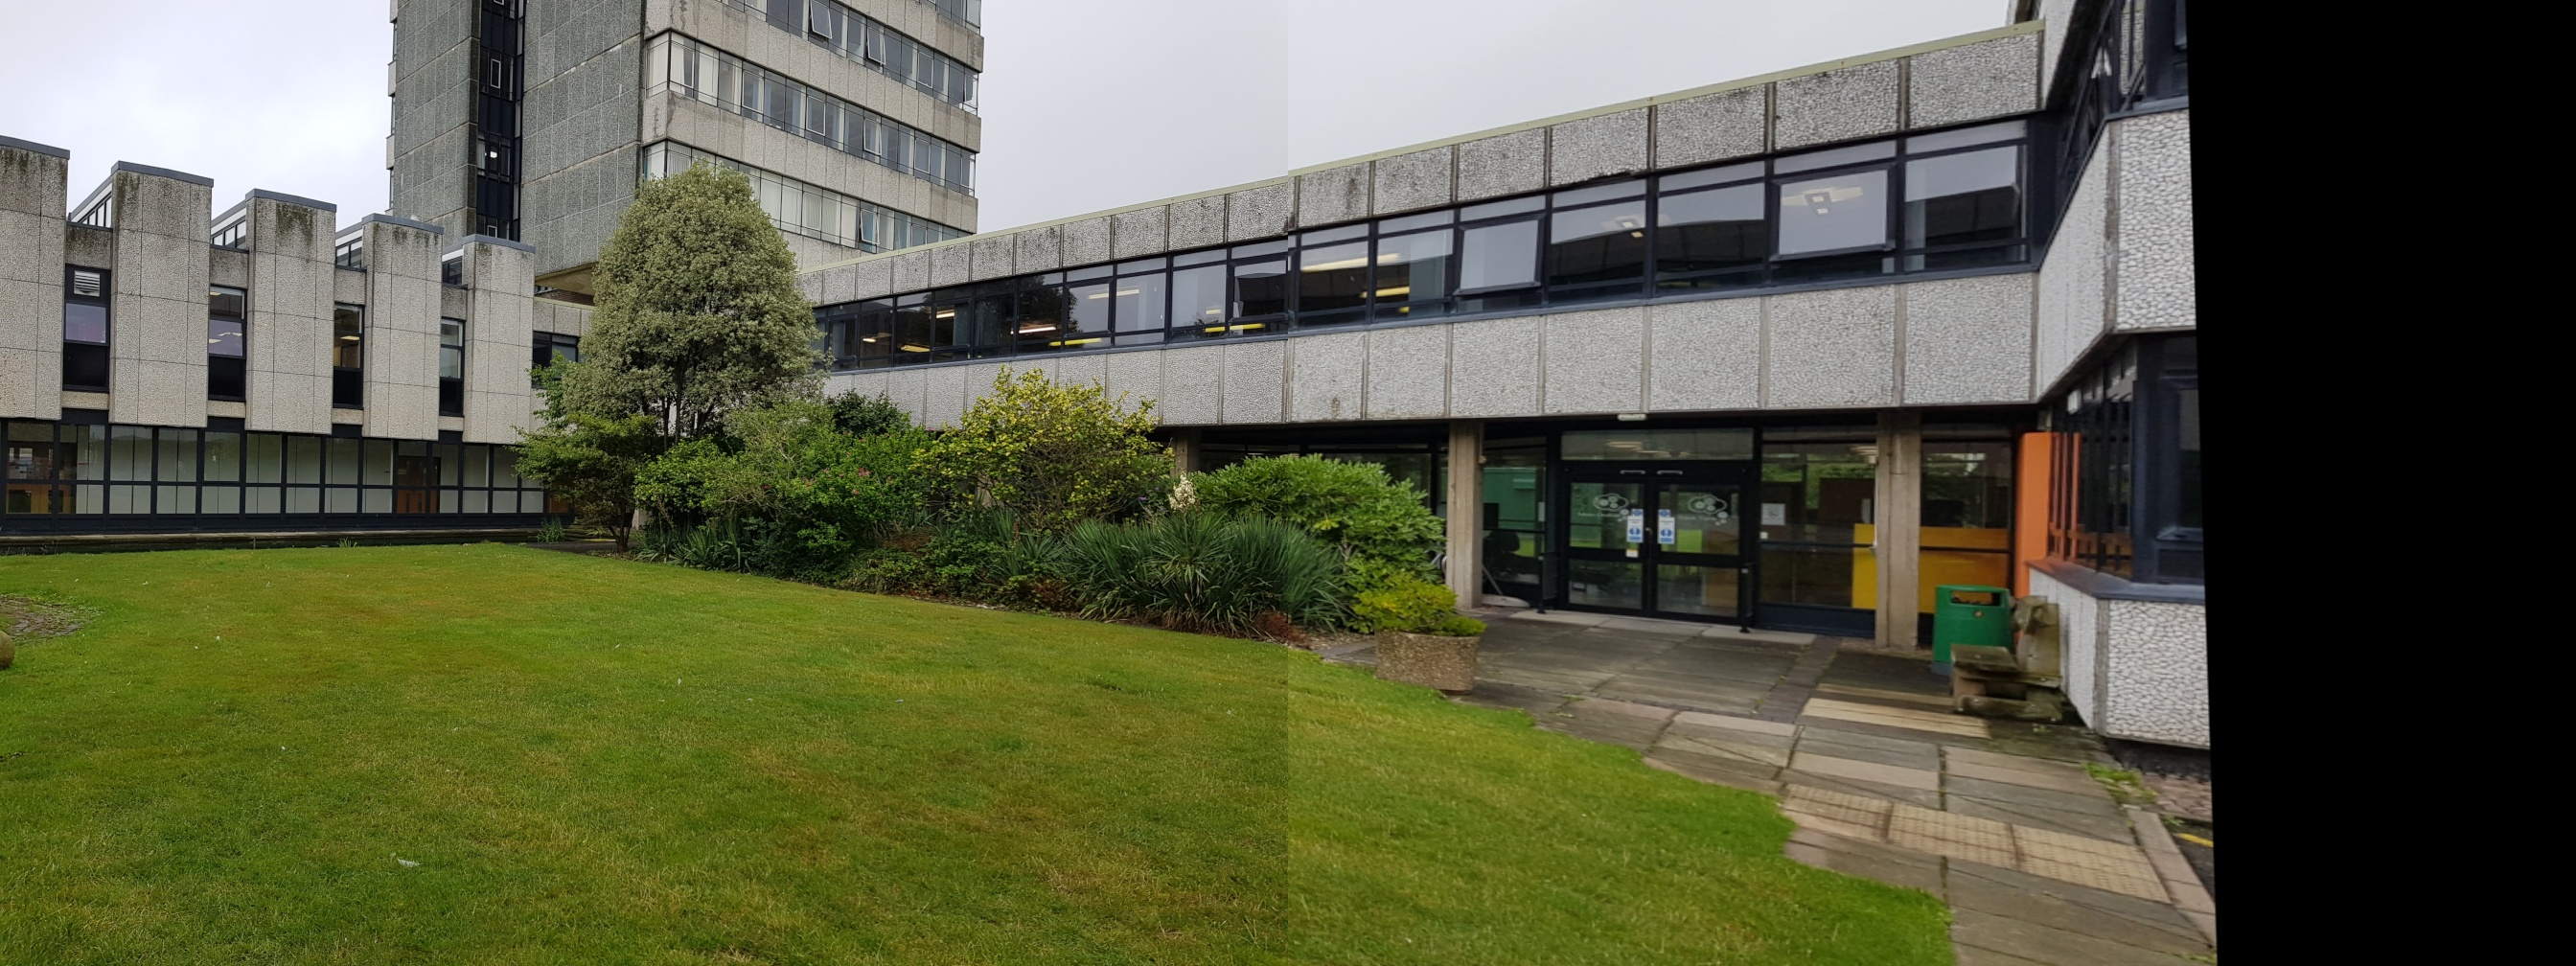
\includegraphics[width=\textwidth]{provided_stitched.jpg}
\caption{provided 拼接结果}
\label{fig:stitch_provided}
\end{figure}

\begin{figure}[H]
\centering
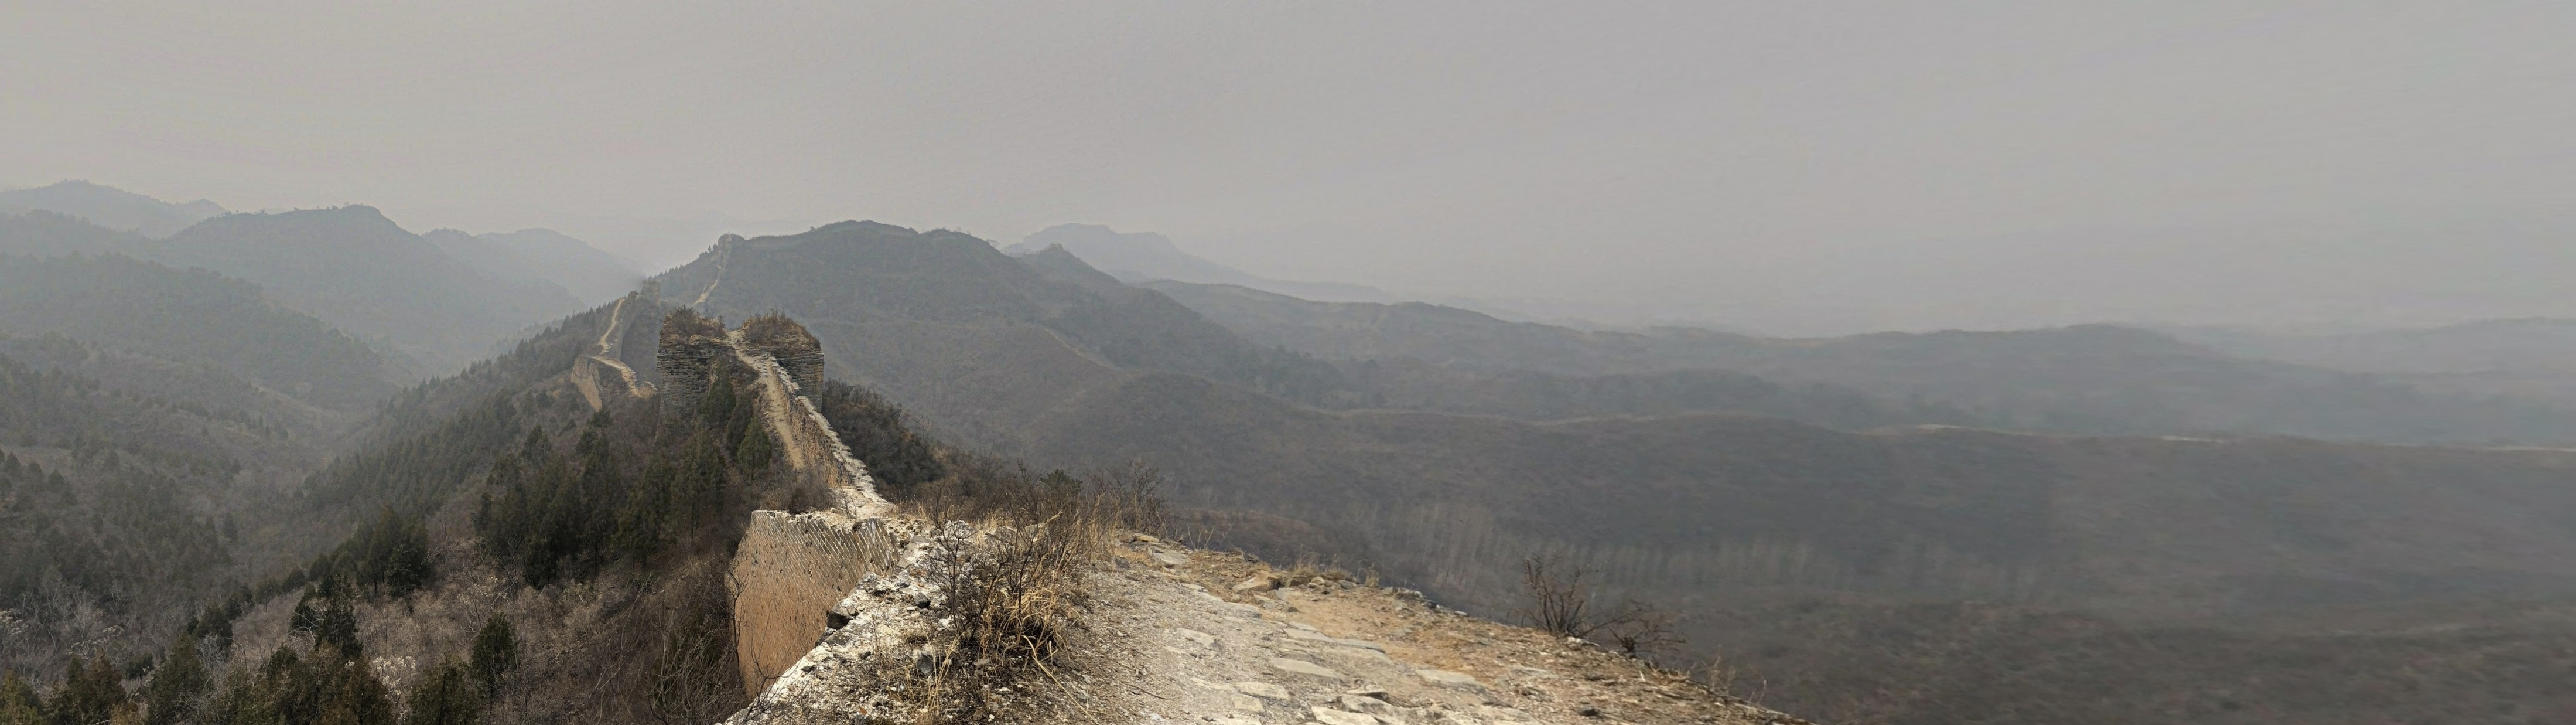
\includegraphics[width=\textwidth]{GreatWall_stitched.jpg}
\caption{GreatWall 拼接结果}
\label{fig:stitch_greatwall}
\end{figure}

\begin{figure}[H]
\centering
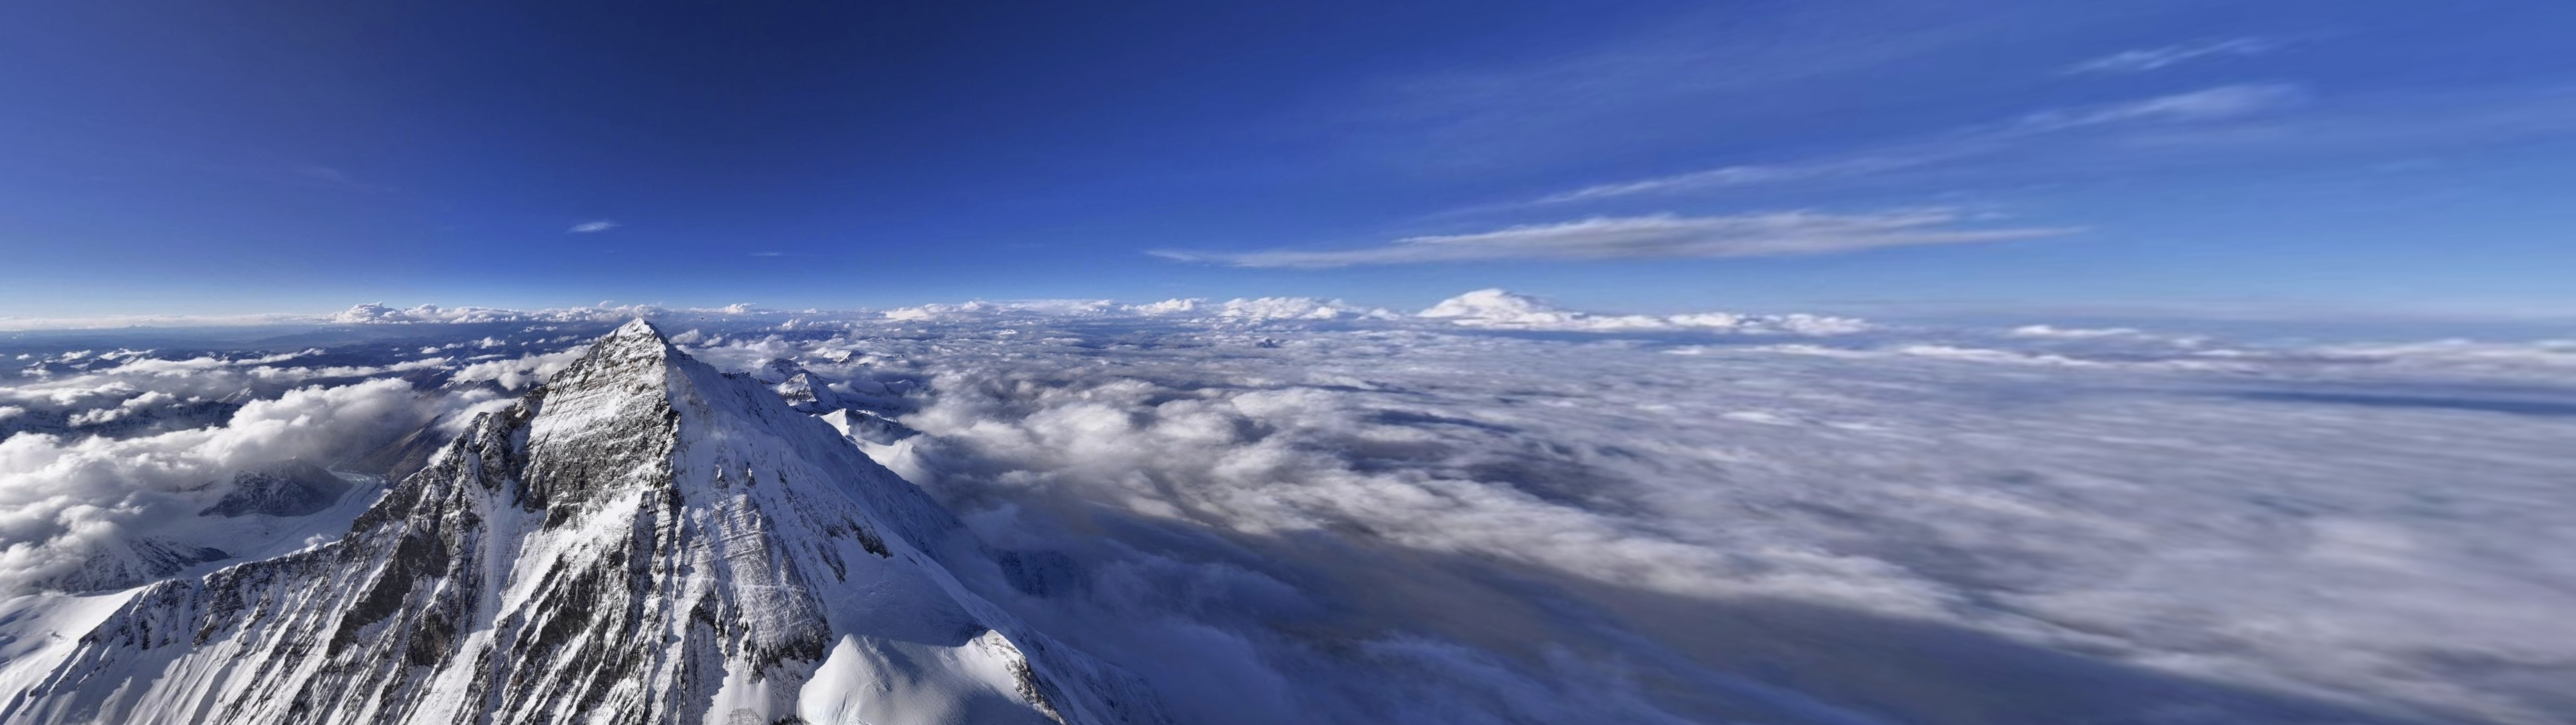
\includegraphics[width=\textwidth]{Everest_stitched.jpg}
\caption{Everest 拼接结果}
\label{fig:stitch_everest}
\end{figure}

\begin{figure}[H]
\centering
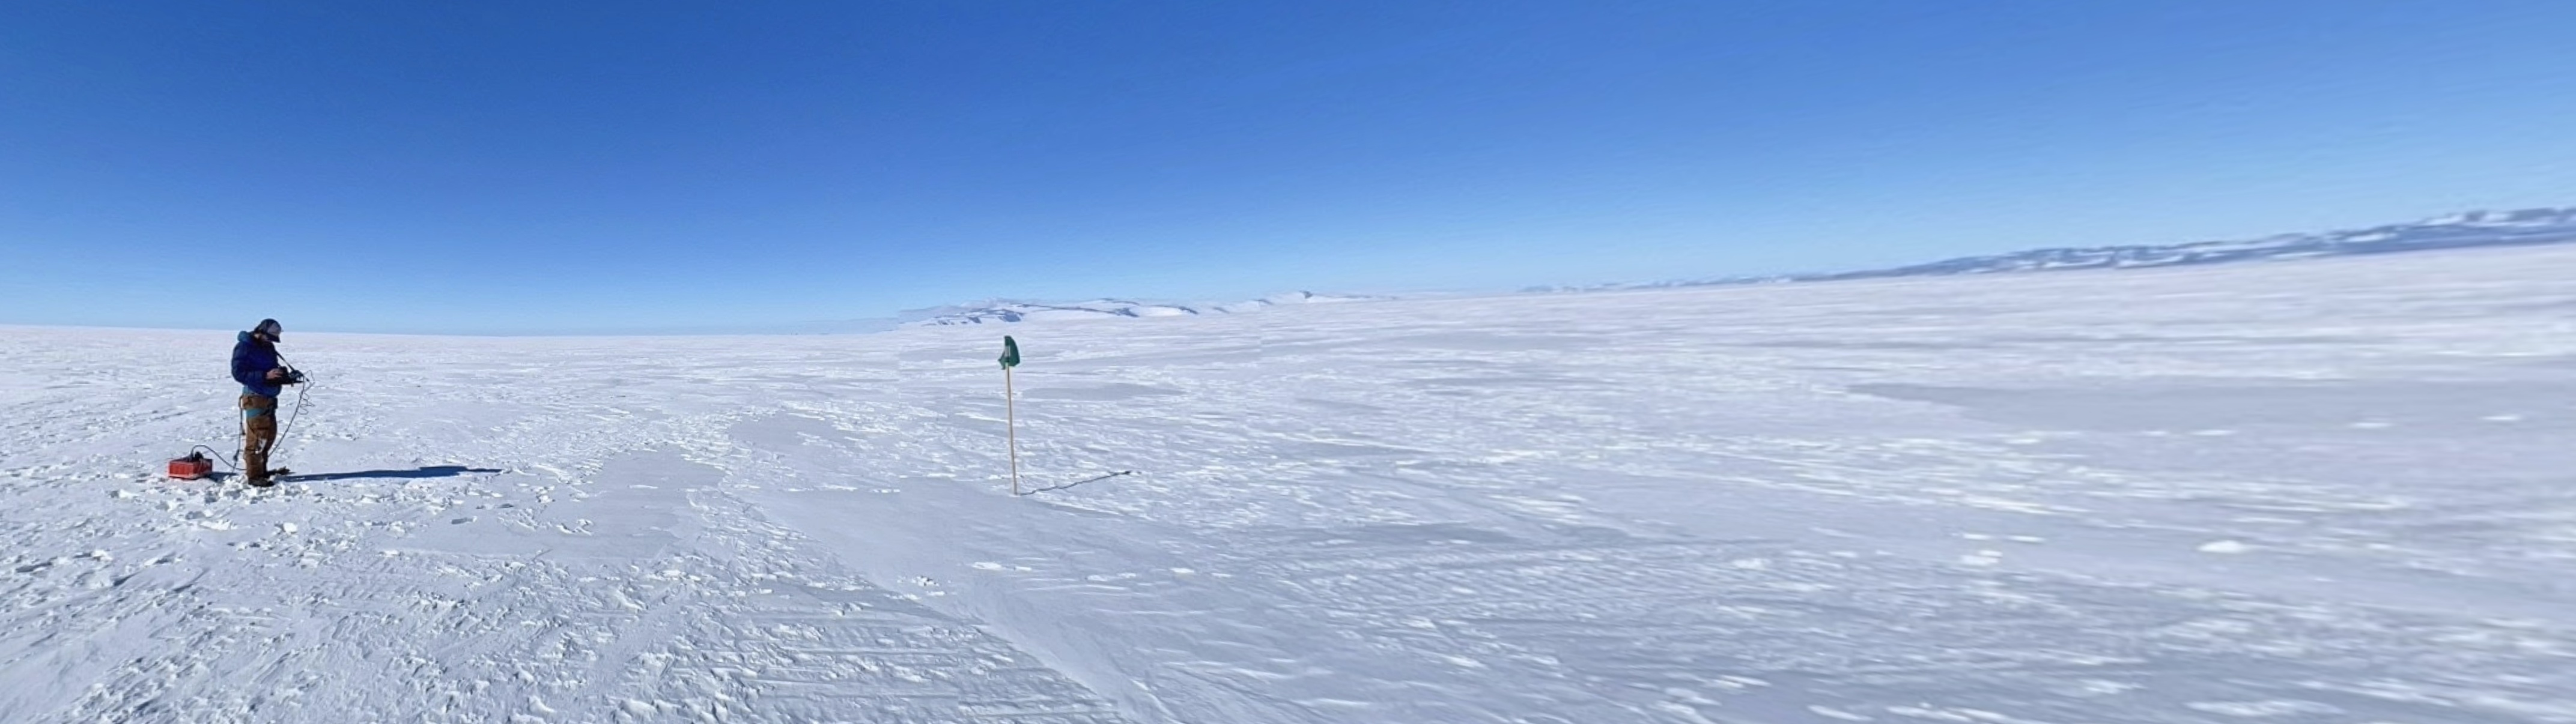
\includegraphics[width=\textwidth]{Antarctica_stitched.jpg}
\caption{Antarctica 拼接结果}
\label{fig:stitch_antarctica}
\end{figure}

\begin{figure}[H]
\centering
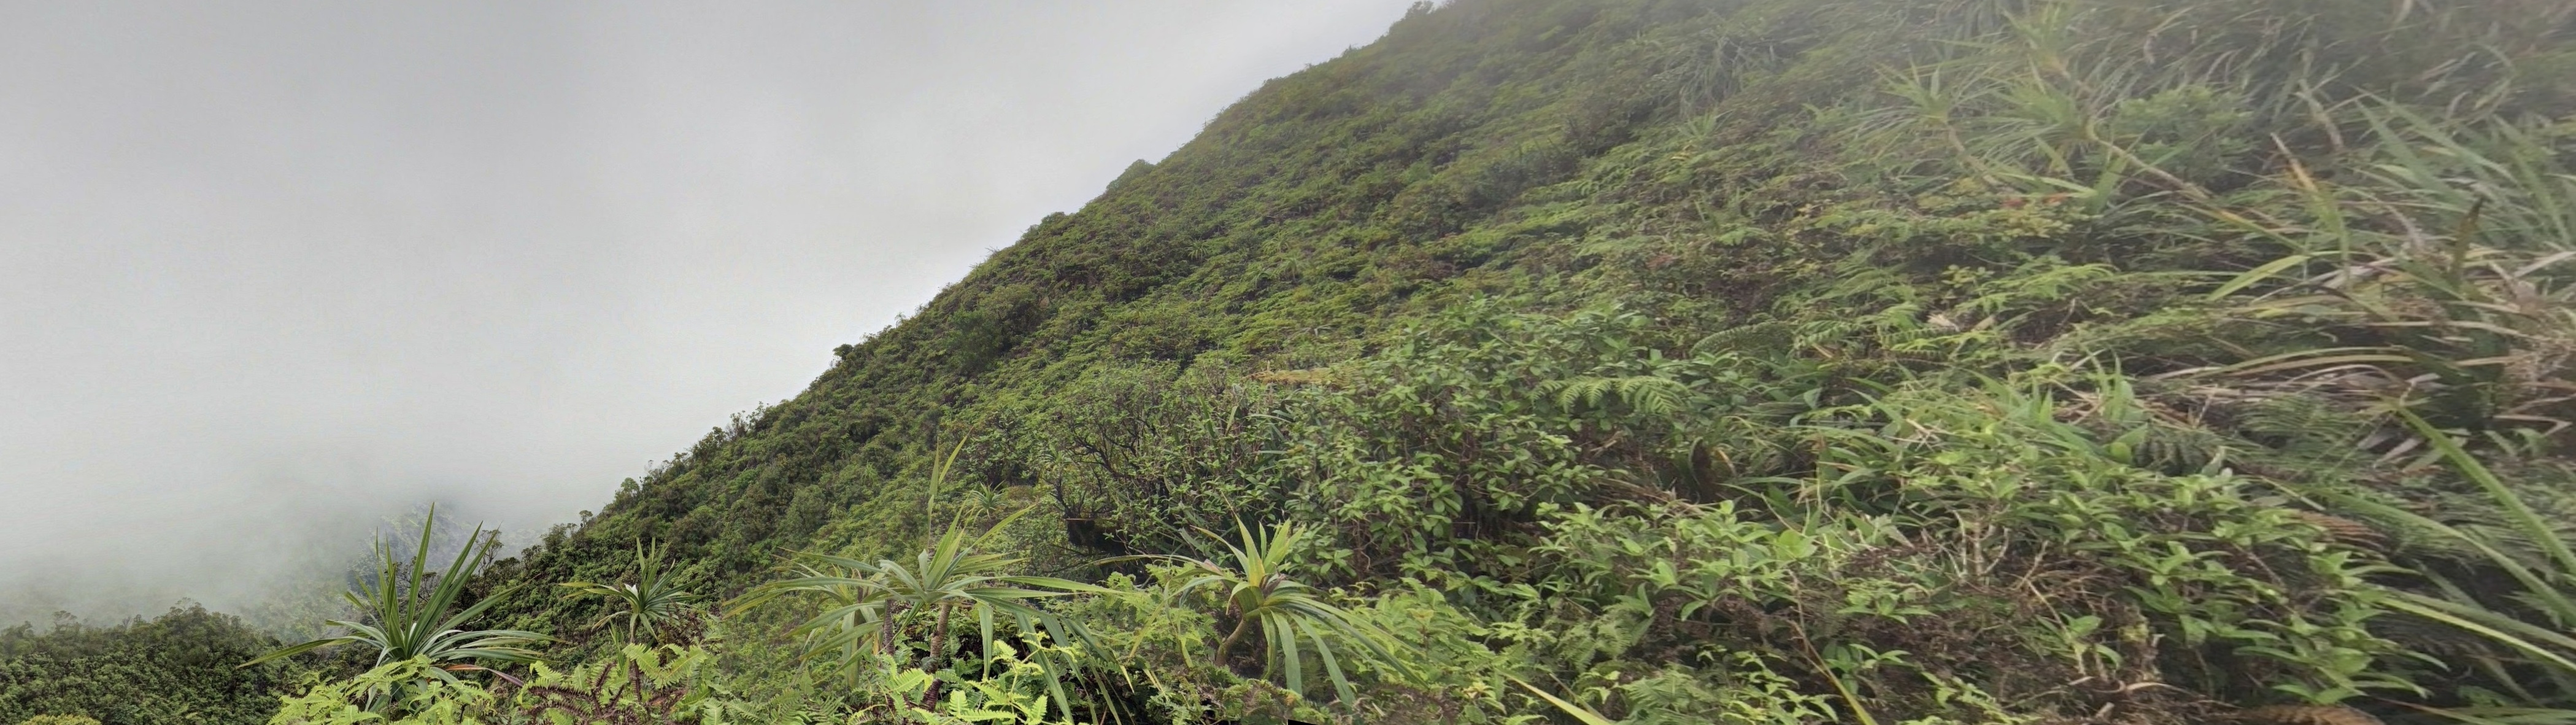
\includegraphics[width=\textwidth]{Honolulu_stitched.jpg}
\caption{Honolulu 拼接结果}
\label{fig:stitch_honolulu}
\end{figure}

\subsubsection{失败案例分析}

\begin{figure}[H]
\centering
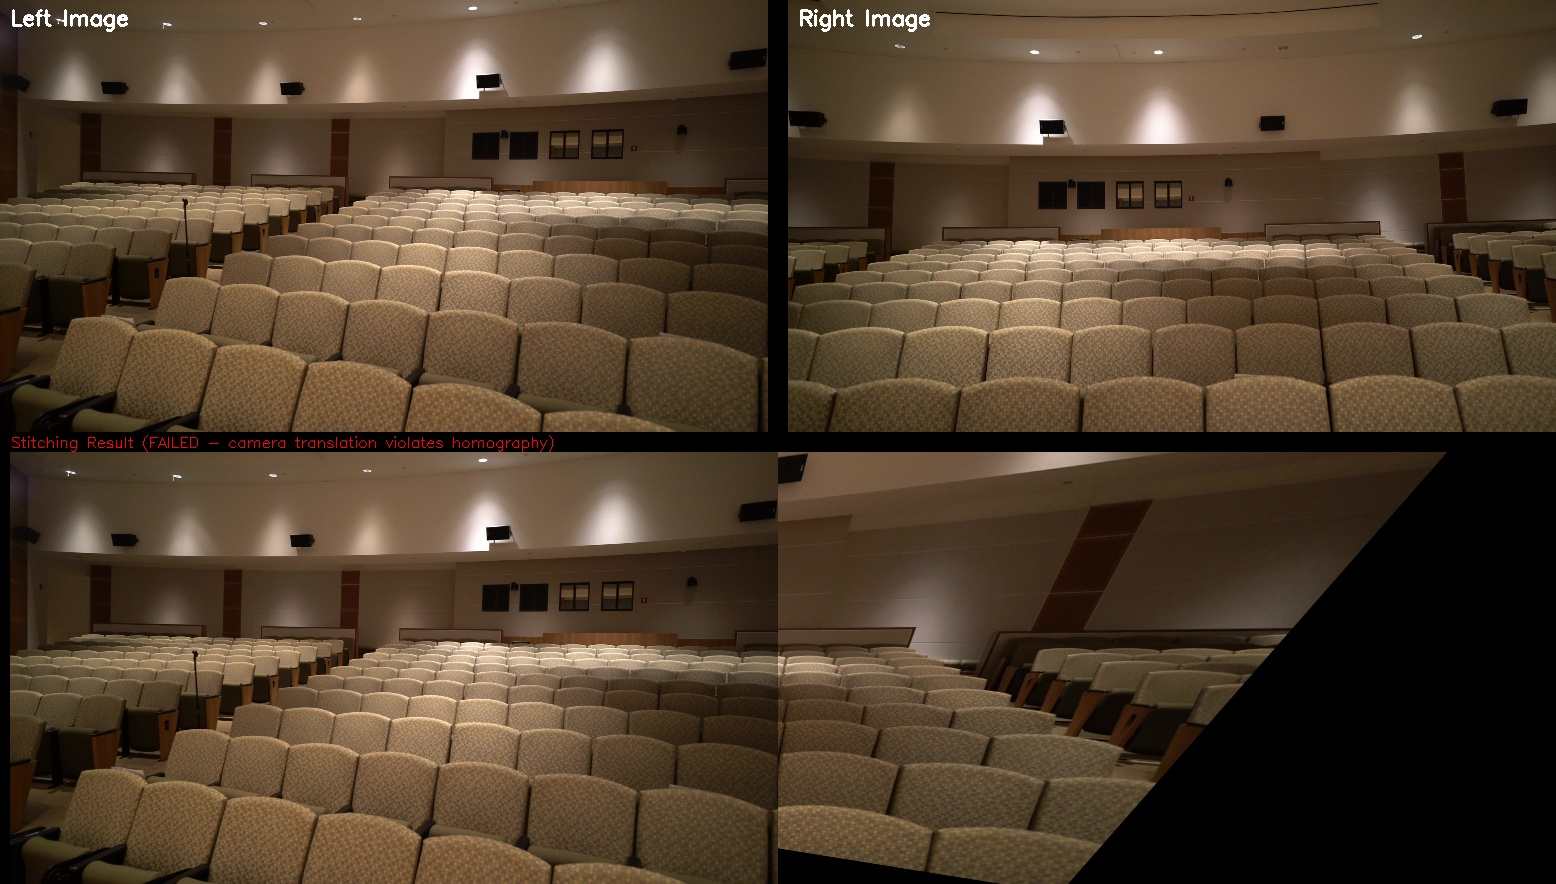
\includegraphics[width=0.9\textwidth]{failure_analysis_Auditorium.jpg}
\caption{Auditorium 拼接案例：室内深度变化导致接缝处出现像素错位}
\label{fig:failure_auditorium}
\end{figure}

\begin{figure}[H]
\centering
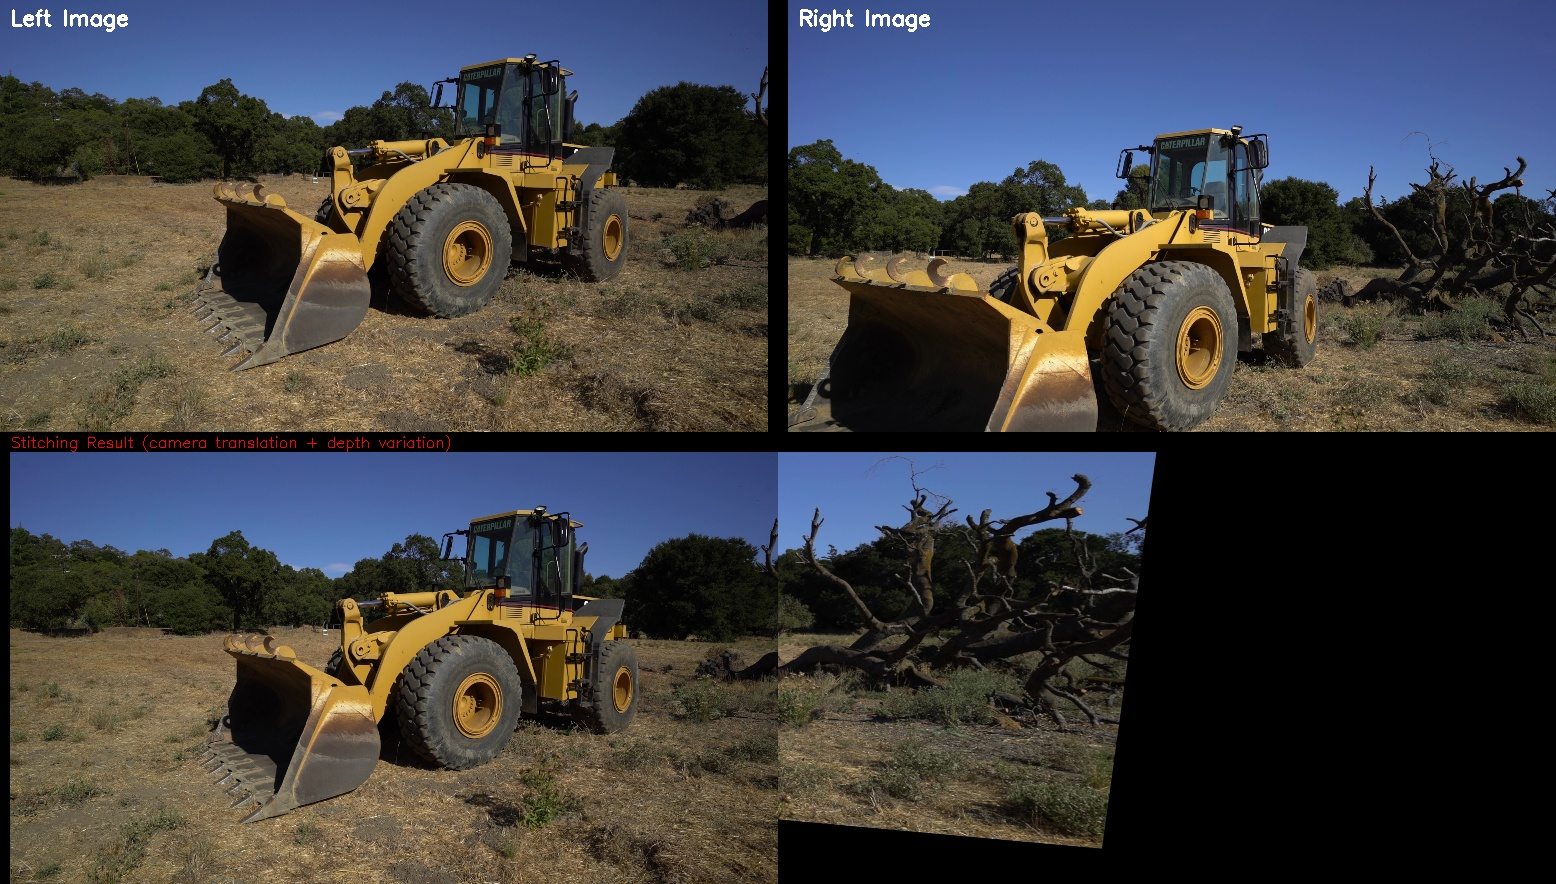
\includegraphics[width=0.9\textwidth]{failure_analysis_Caterpillar.jpg}
\caption{Caterpillar 拼接案例：室内深度变化导致接缝处出现像素错位}
\label{fig:failure_caterpillar}
\end{figure}

\begin{figure}[H]
\centering
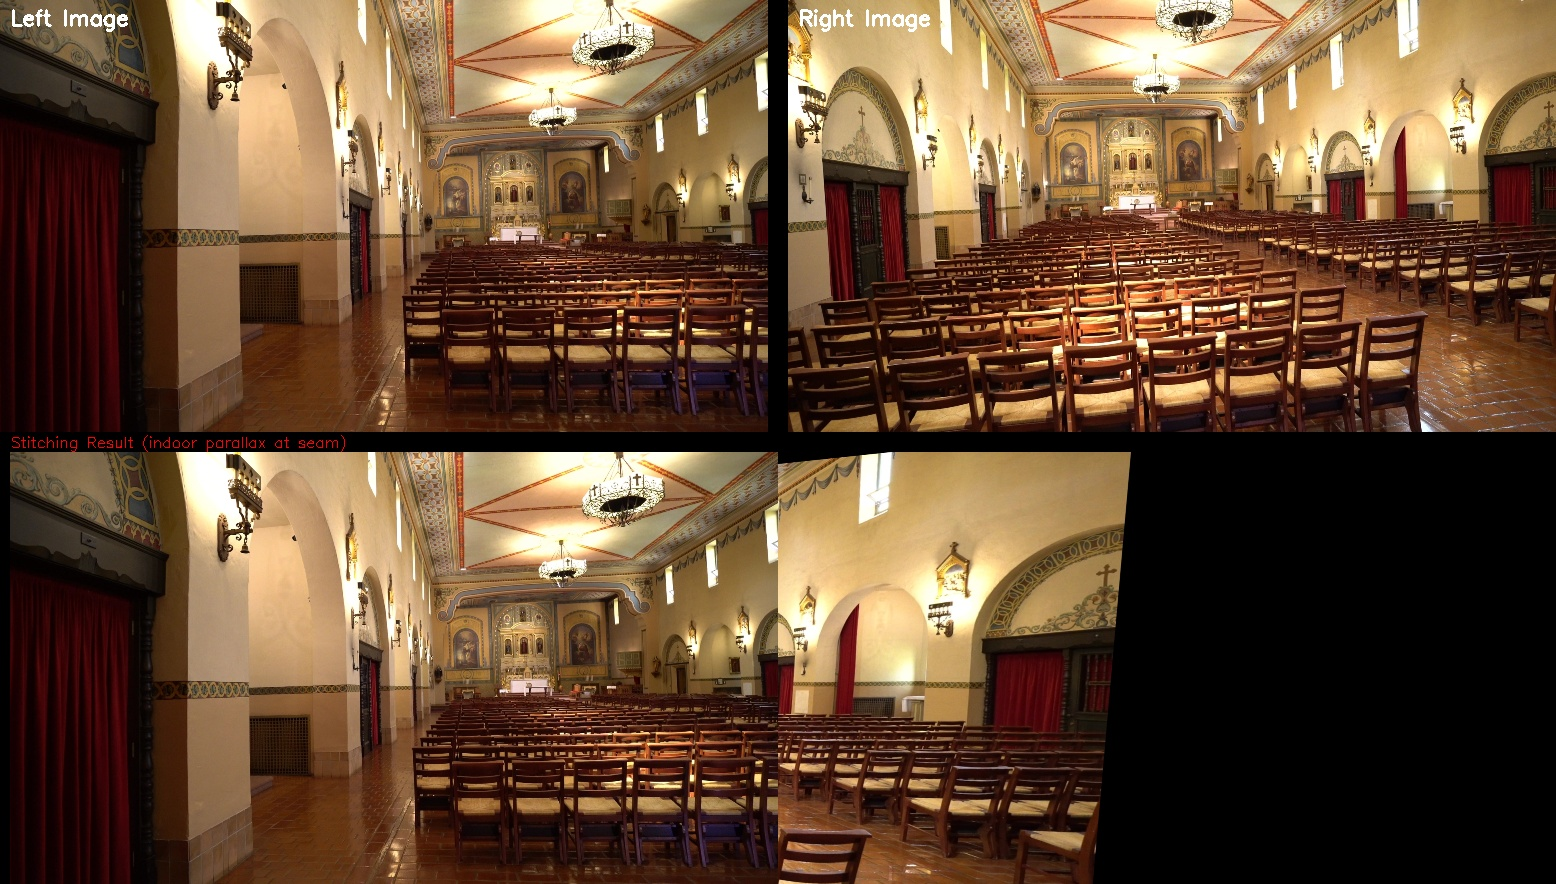
\includegraphics[width=0.9\textwidth]{failure_analysis_Church.jpg}
\caption{Church 拼接案例：室内深度变化导致接缝处出现像素错位}
\label{fig:failure_church}
\end{figure}

\begin{figure}[H]
\centering
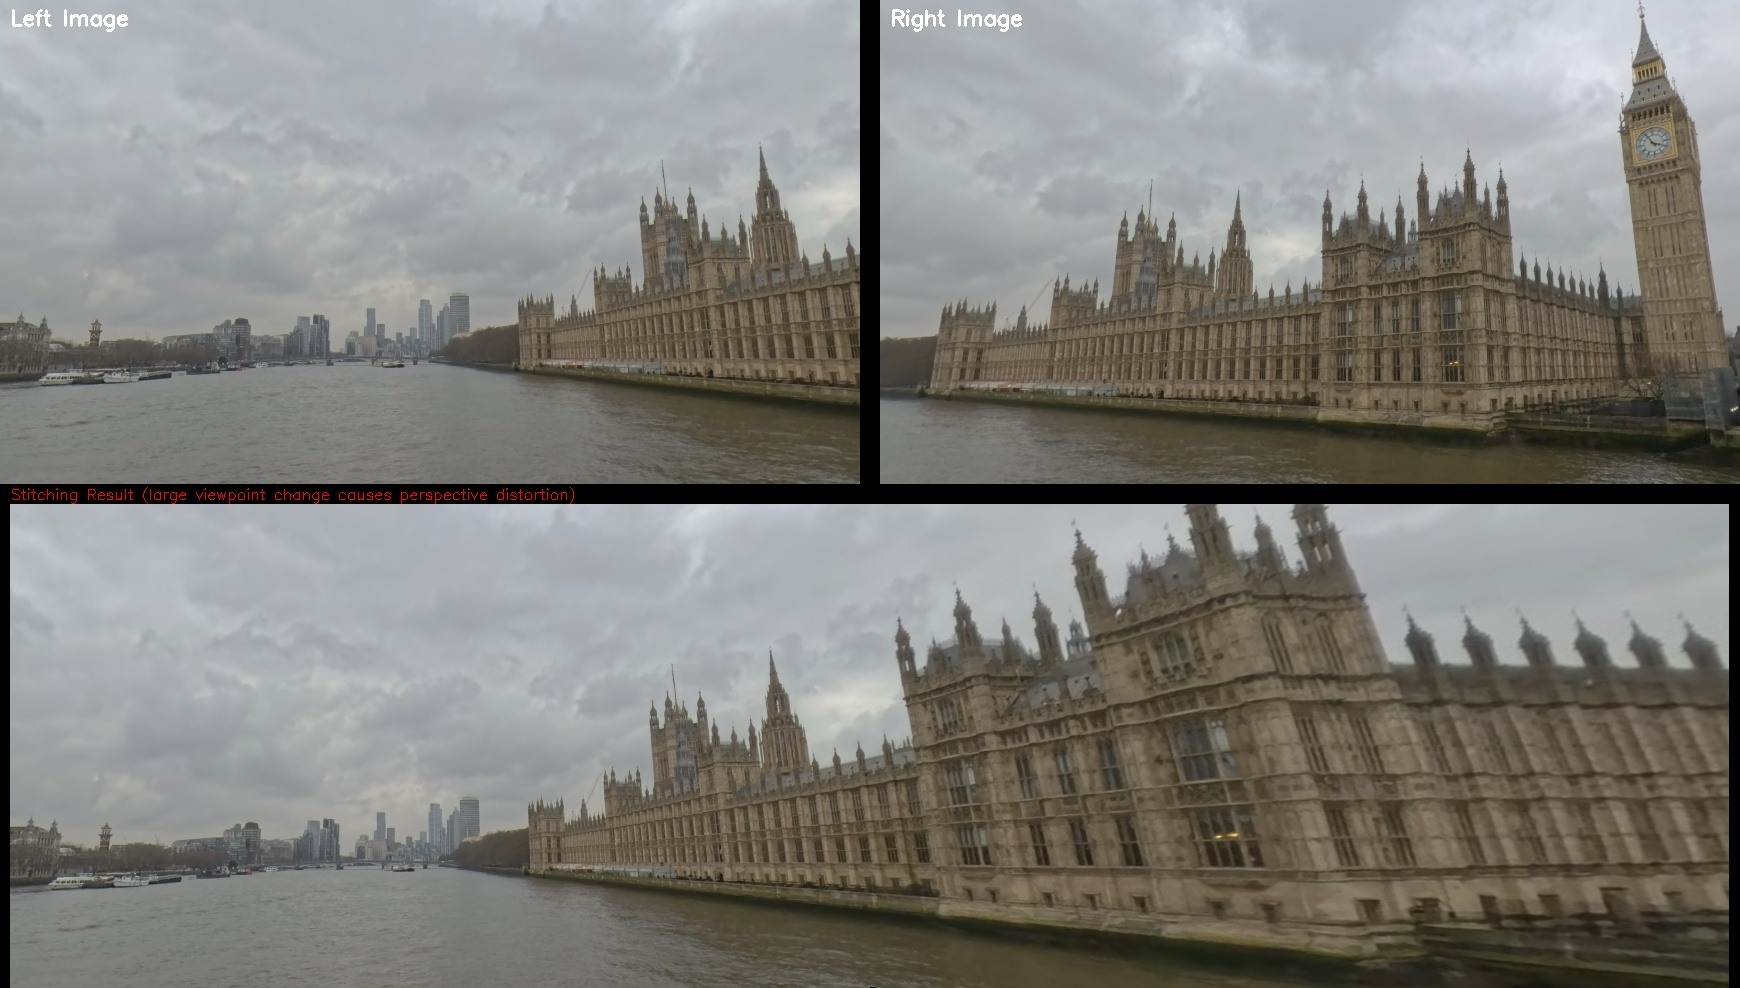
\includegraphics[width=0.9\textwidth]{failure_analysis_BigBen.jpg}
\caption{BigBen 拼接案例：大视角变化导致右侧透视拉伸严重（已截取掉超出画幅的部分）}
\label{fig:failure_bigben}
\end{figure}

如图\ref{fig:failure_auditorium}--\ref{fig:failure_bigben}所示，四组困难场景的拼接结果展现了不同类型的伪影，其成因各有侧重。

Auditorium（图\ref{fig:failure_auditorium}）的问题主要来自重复纹理导致的匹配歧义。场景中大面积重复的座椅纹理使得RANSAC内点率仅为45\%，超过一半的匹配对为错误匹配，由此估计的单应性矩阵不够准确，warp后的右图在边缘区域出现明显的几何变形。

Caterpillar（图\ref{fig:failure_caterpillar}）的失败源于场景的深度不一致。推土机前景与远处树林背景之间的深度差异巨大，不同深度的物体严格来说对应不同的单应性变换，用单一矩阵拟合必然导致至少一个深度层出现明显错位。

Church（图\ref{fig:failure_church}）的拼接结果整体正确，但在左右图像的接缝处可观察到明显的像素错位。这同样源于室内场景的深度变化——教堂的前排椅子与后方祭坛处于不同的深度平面，单应性拼接在它们之间产生了不可调和的几何矛盾。

BigBen（图\ref{fig:failure_bigben}）则展示了大视角变化带来的透视拉伸问题。当两幅图像之间的旋转角度较大时，透视变换会将远离重叠区域的图像内容极端拉伸，导致右侧边缘出现严重的几何畸变。这是透视投影模型的固有数学性质，在大视角场景下不可避免。

\subsection{局限}

当前系统存在若干局限性，为未来改进提供了明确的方向。

在图像融合方面，当前采用的简单覆盖策略在重叠区域会产生可见的亮度跳变和硬接缝，影响全景图的视觉质量；在几何模型方面，单应性变换仅能正确描述平面场景或纯旋转相机的情况。当场景存在明显的深度变化且相机有平移运动时，应考虑使用基本矩阵进行立体几何建模，或采用多模型拟合（如PEARL算法）来处理包含多个平面的复杂场景；在画布利用方面，按作业要求固定画布宽度为$w_1 + w_2$，在两幅图重叠度较高时会导致画布右侧出现大面积黑色空白区域。实际应用中可根据warp后右图角点的实际坐标范围自适应地确定画布大小，以提高空间利用效率。

% ============================================================
\section{用户界面与实拍测试}

\subsection{用户界面设计}

为方便可视化调试和结果展示，本系统实现了基于Tkinter的图形用户界面。界面顶部的控制面板提供了7个功能按钮，用户可以按照流水线顺序逐步执行各阶段操作。界面中部左右两侧分别显示左图和右图的处理结果，底部的结果区域用于展示特征匹配连线图和最终拼接全景图。

系统支持两种图像加载方式：通过「加载预设图像」按钮可从项目数据目录中选取已有的图像对；通过「自选图像对」按钮则允许用户通过文件对话框自由选取任意两张图片进行拼接，以测试系统在未知数据上的泛化能力。

\subsection{实拍数据测试}

为验证系统在真实场景下的表现，作者使用手机在实验室内拍摄了一对测试图像（图\ref{fig:test_pair}），场景包含门和桌面物品等多种纹理结构。

\begin{figure}[H]
\centering
\begin{subfigure}[b]{0.48\textwidth}
    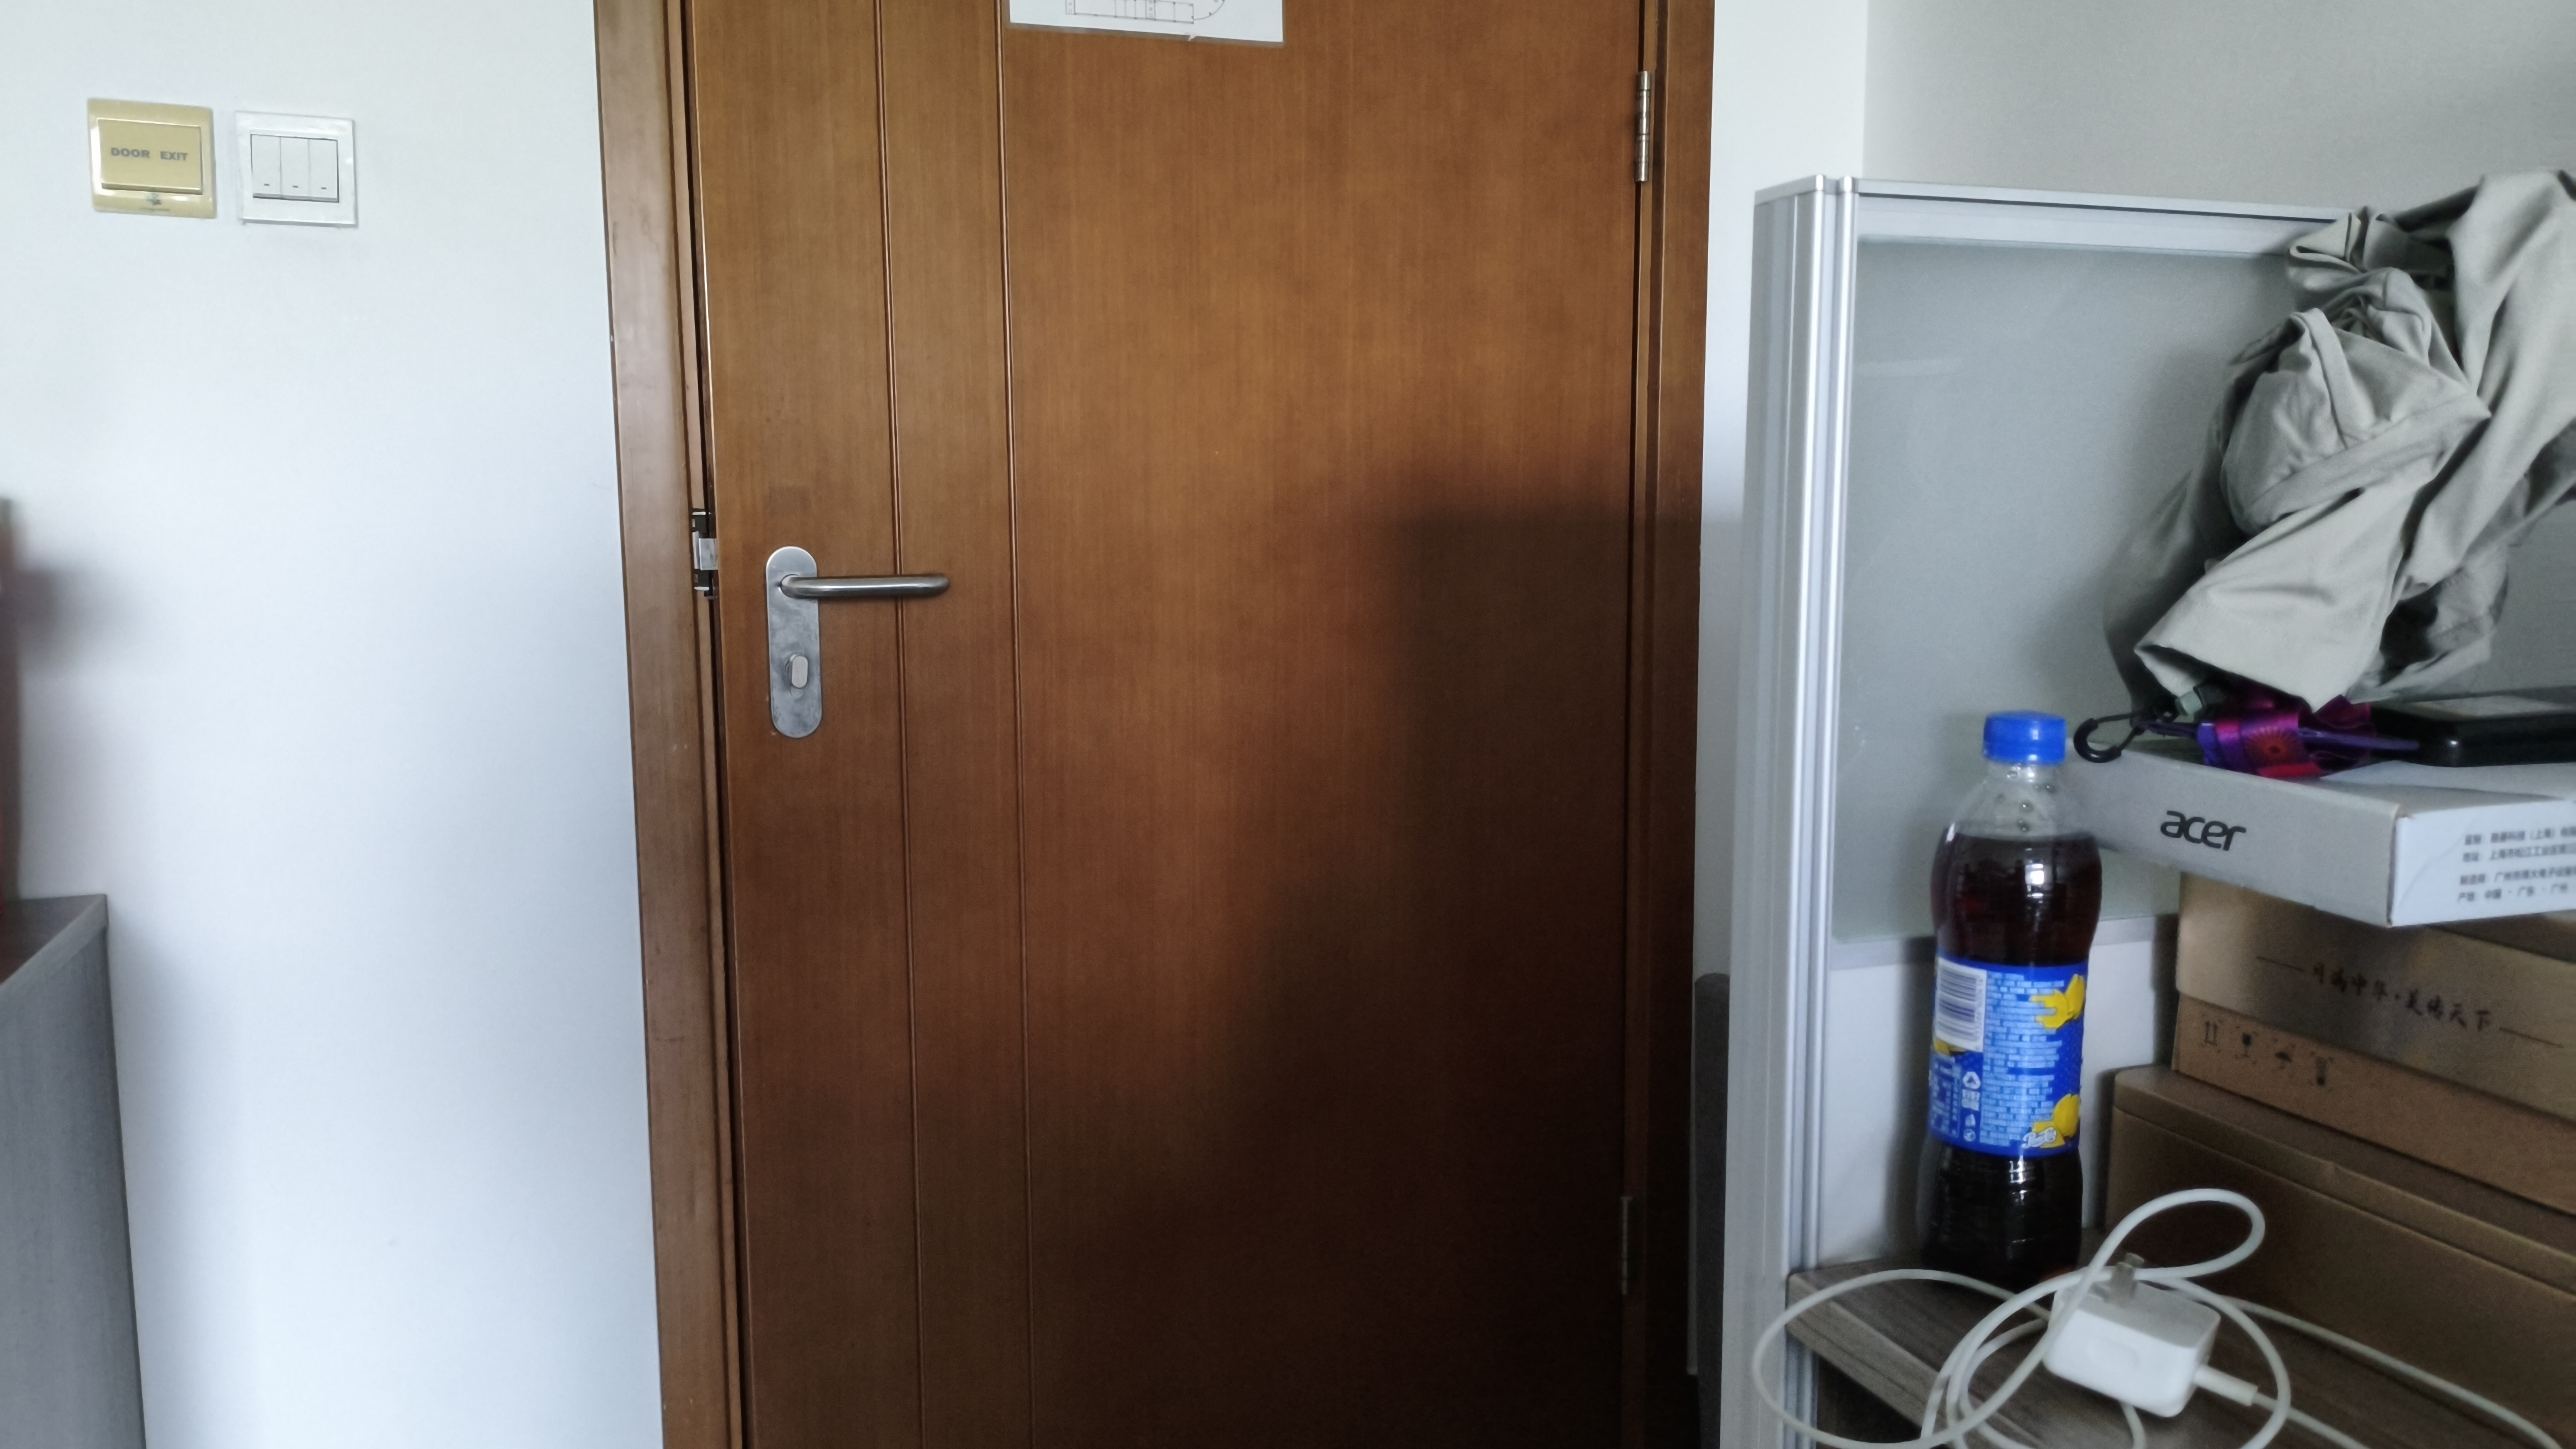
\includegraphics[width=\textwidth]{../data/test/left.jpg}
    \caption{左图}
\end{subfigure}
\hfill
\begin{subfigure}[b]{0.48\textwidth}
    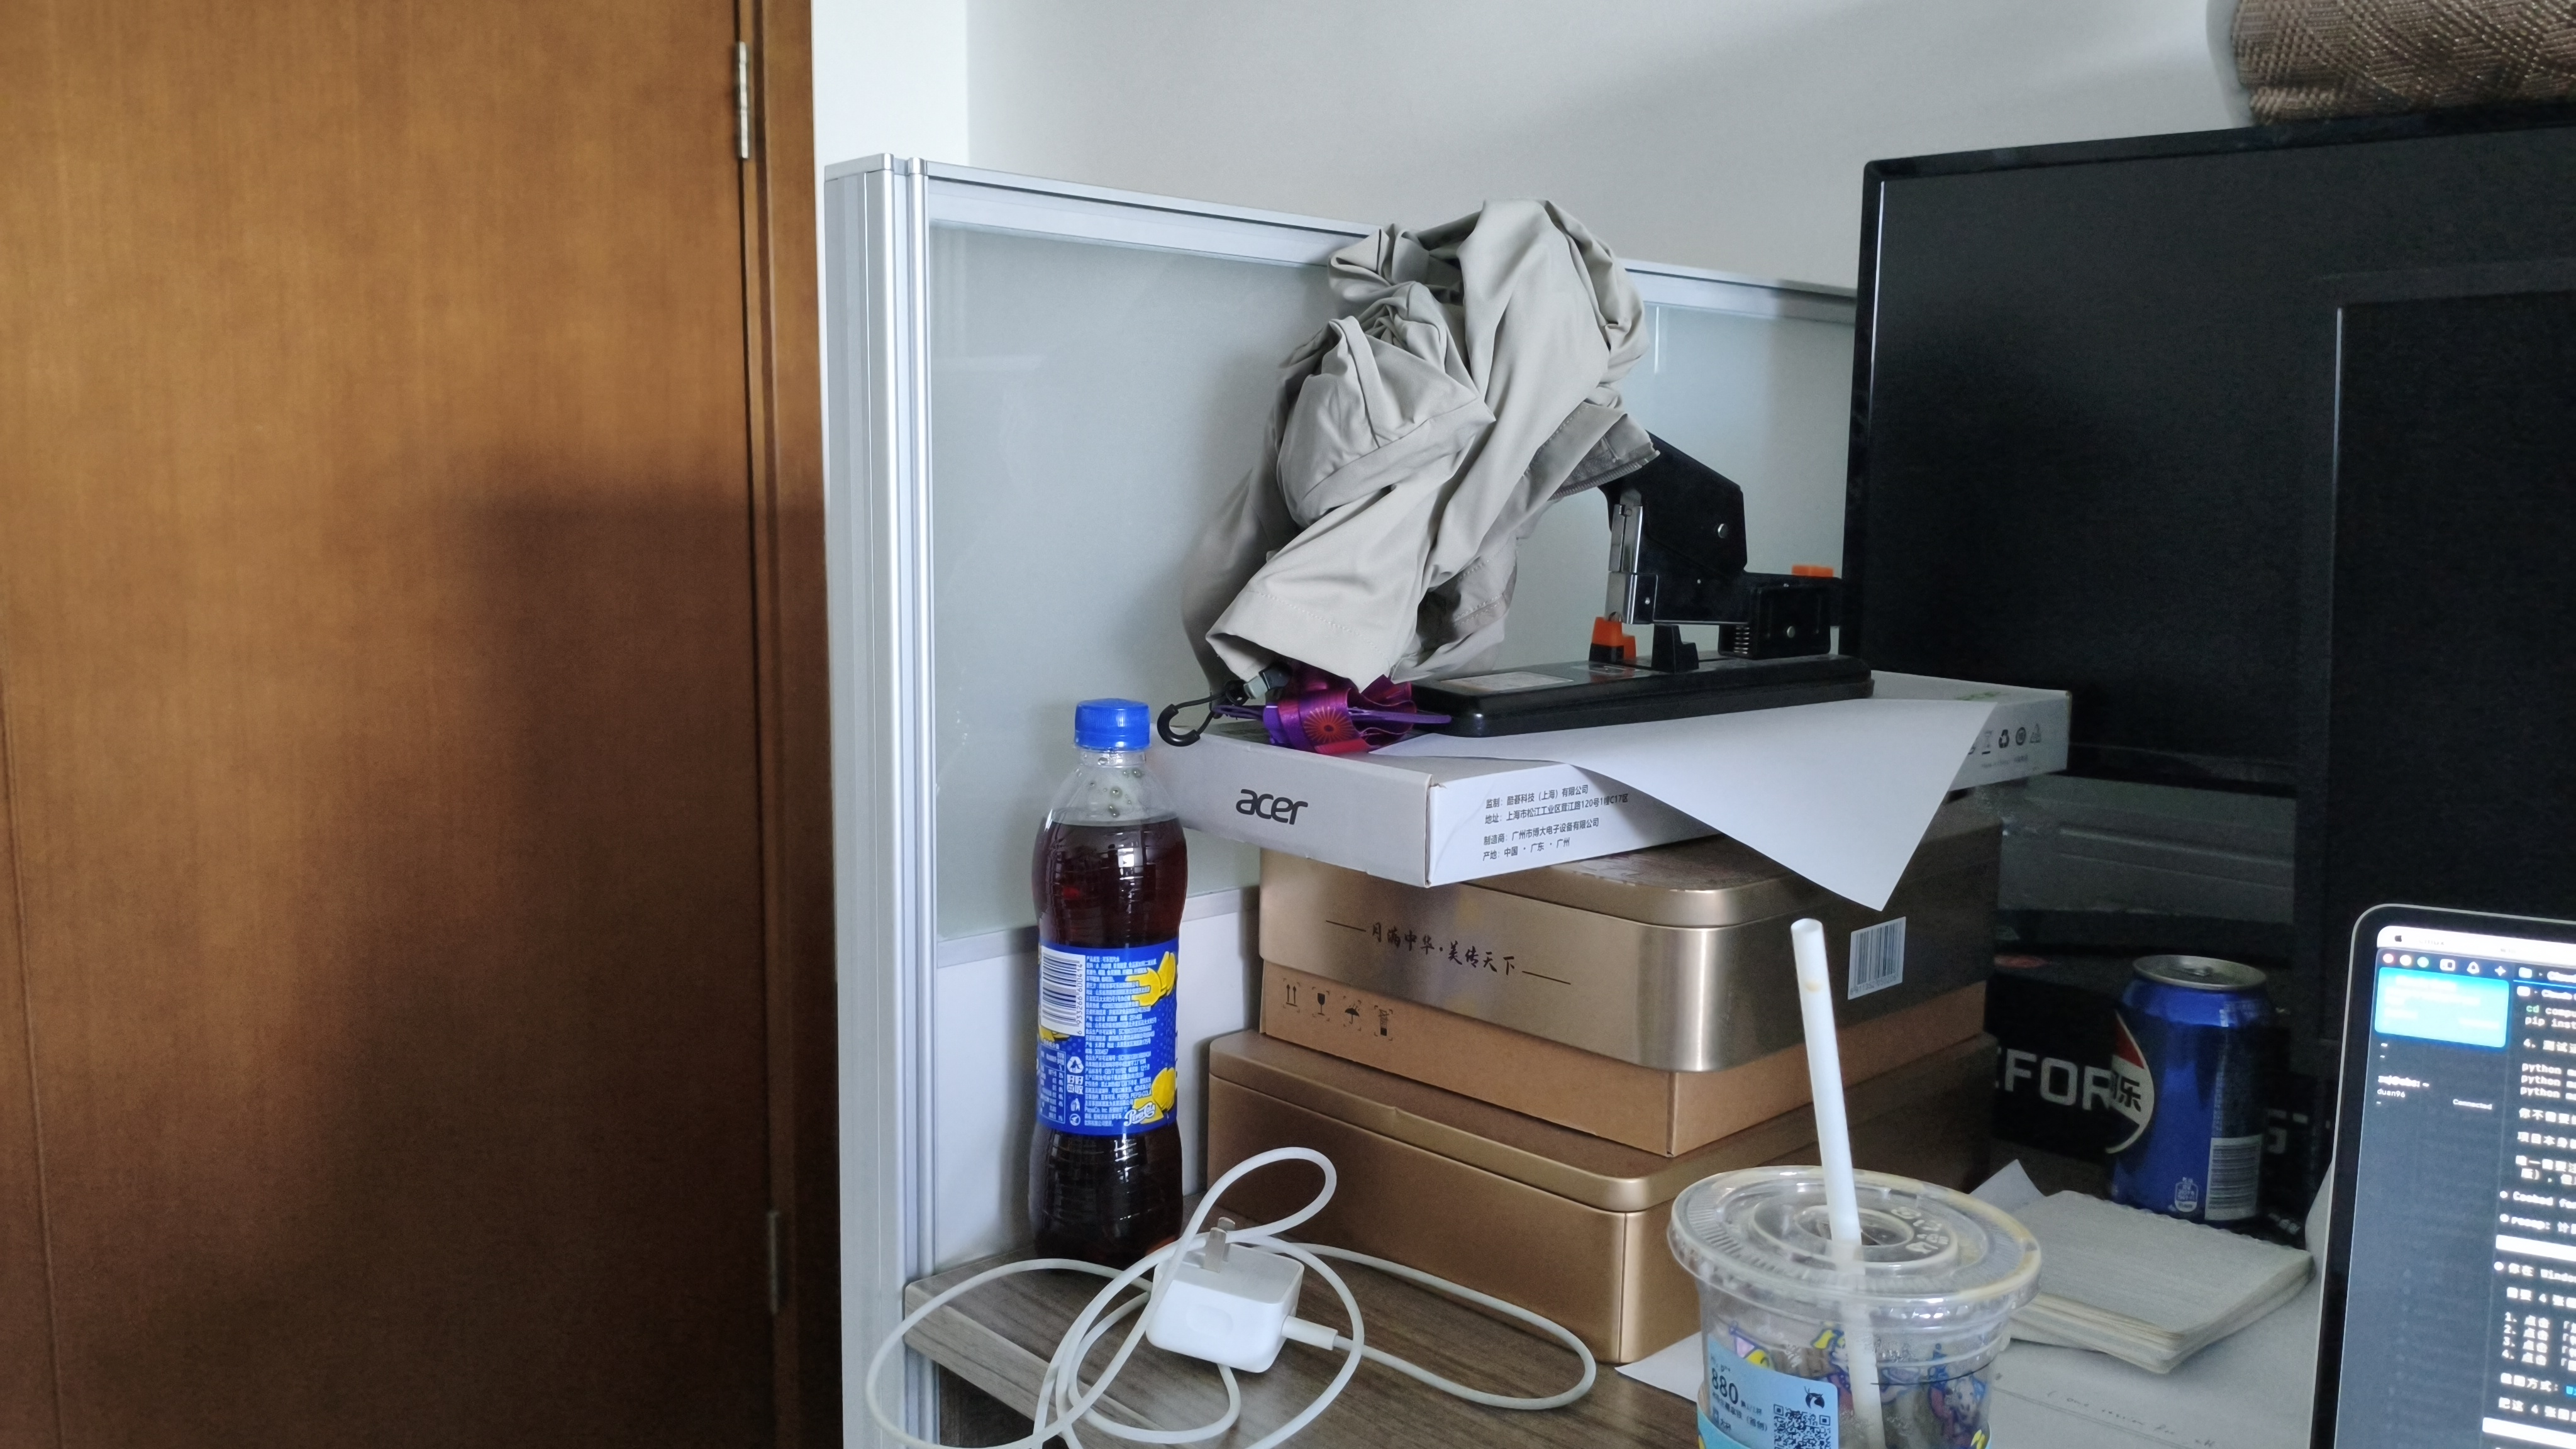
\includegraphics[width=\textwidth]{../data/test/right.jpg}
    \caption{右图}
\end{subfigure}
\caption{实验室实拍测试图像对}
\label{fig:test_pair}
\end{figure}

\subsection{GUI操作流程演示}

图\ref{fig:gui_load}--\ref{fig:gui_stitch}展示了使用GUI界面对实拍数据进行完整拼接流程的四个阶段。用户通过「自选图像对」按钮加载了实验室拍摄的左右图像后，依次执行特征检测、特征匹配和图像拼接操作。

\begin{figure}[H]
\centering
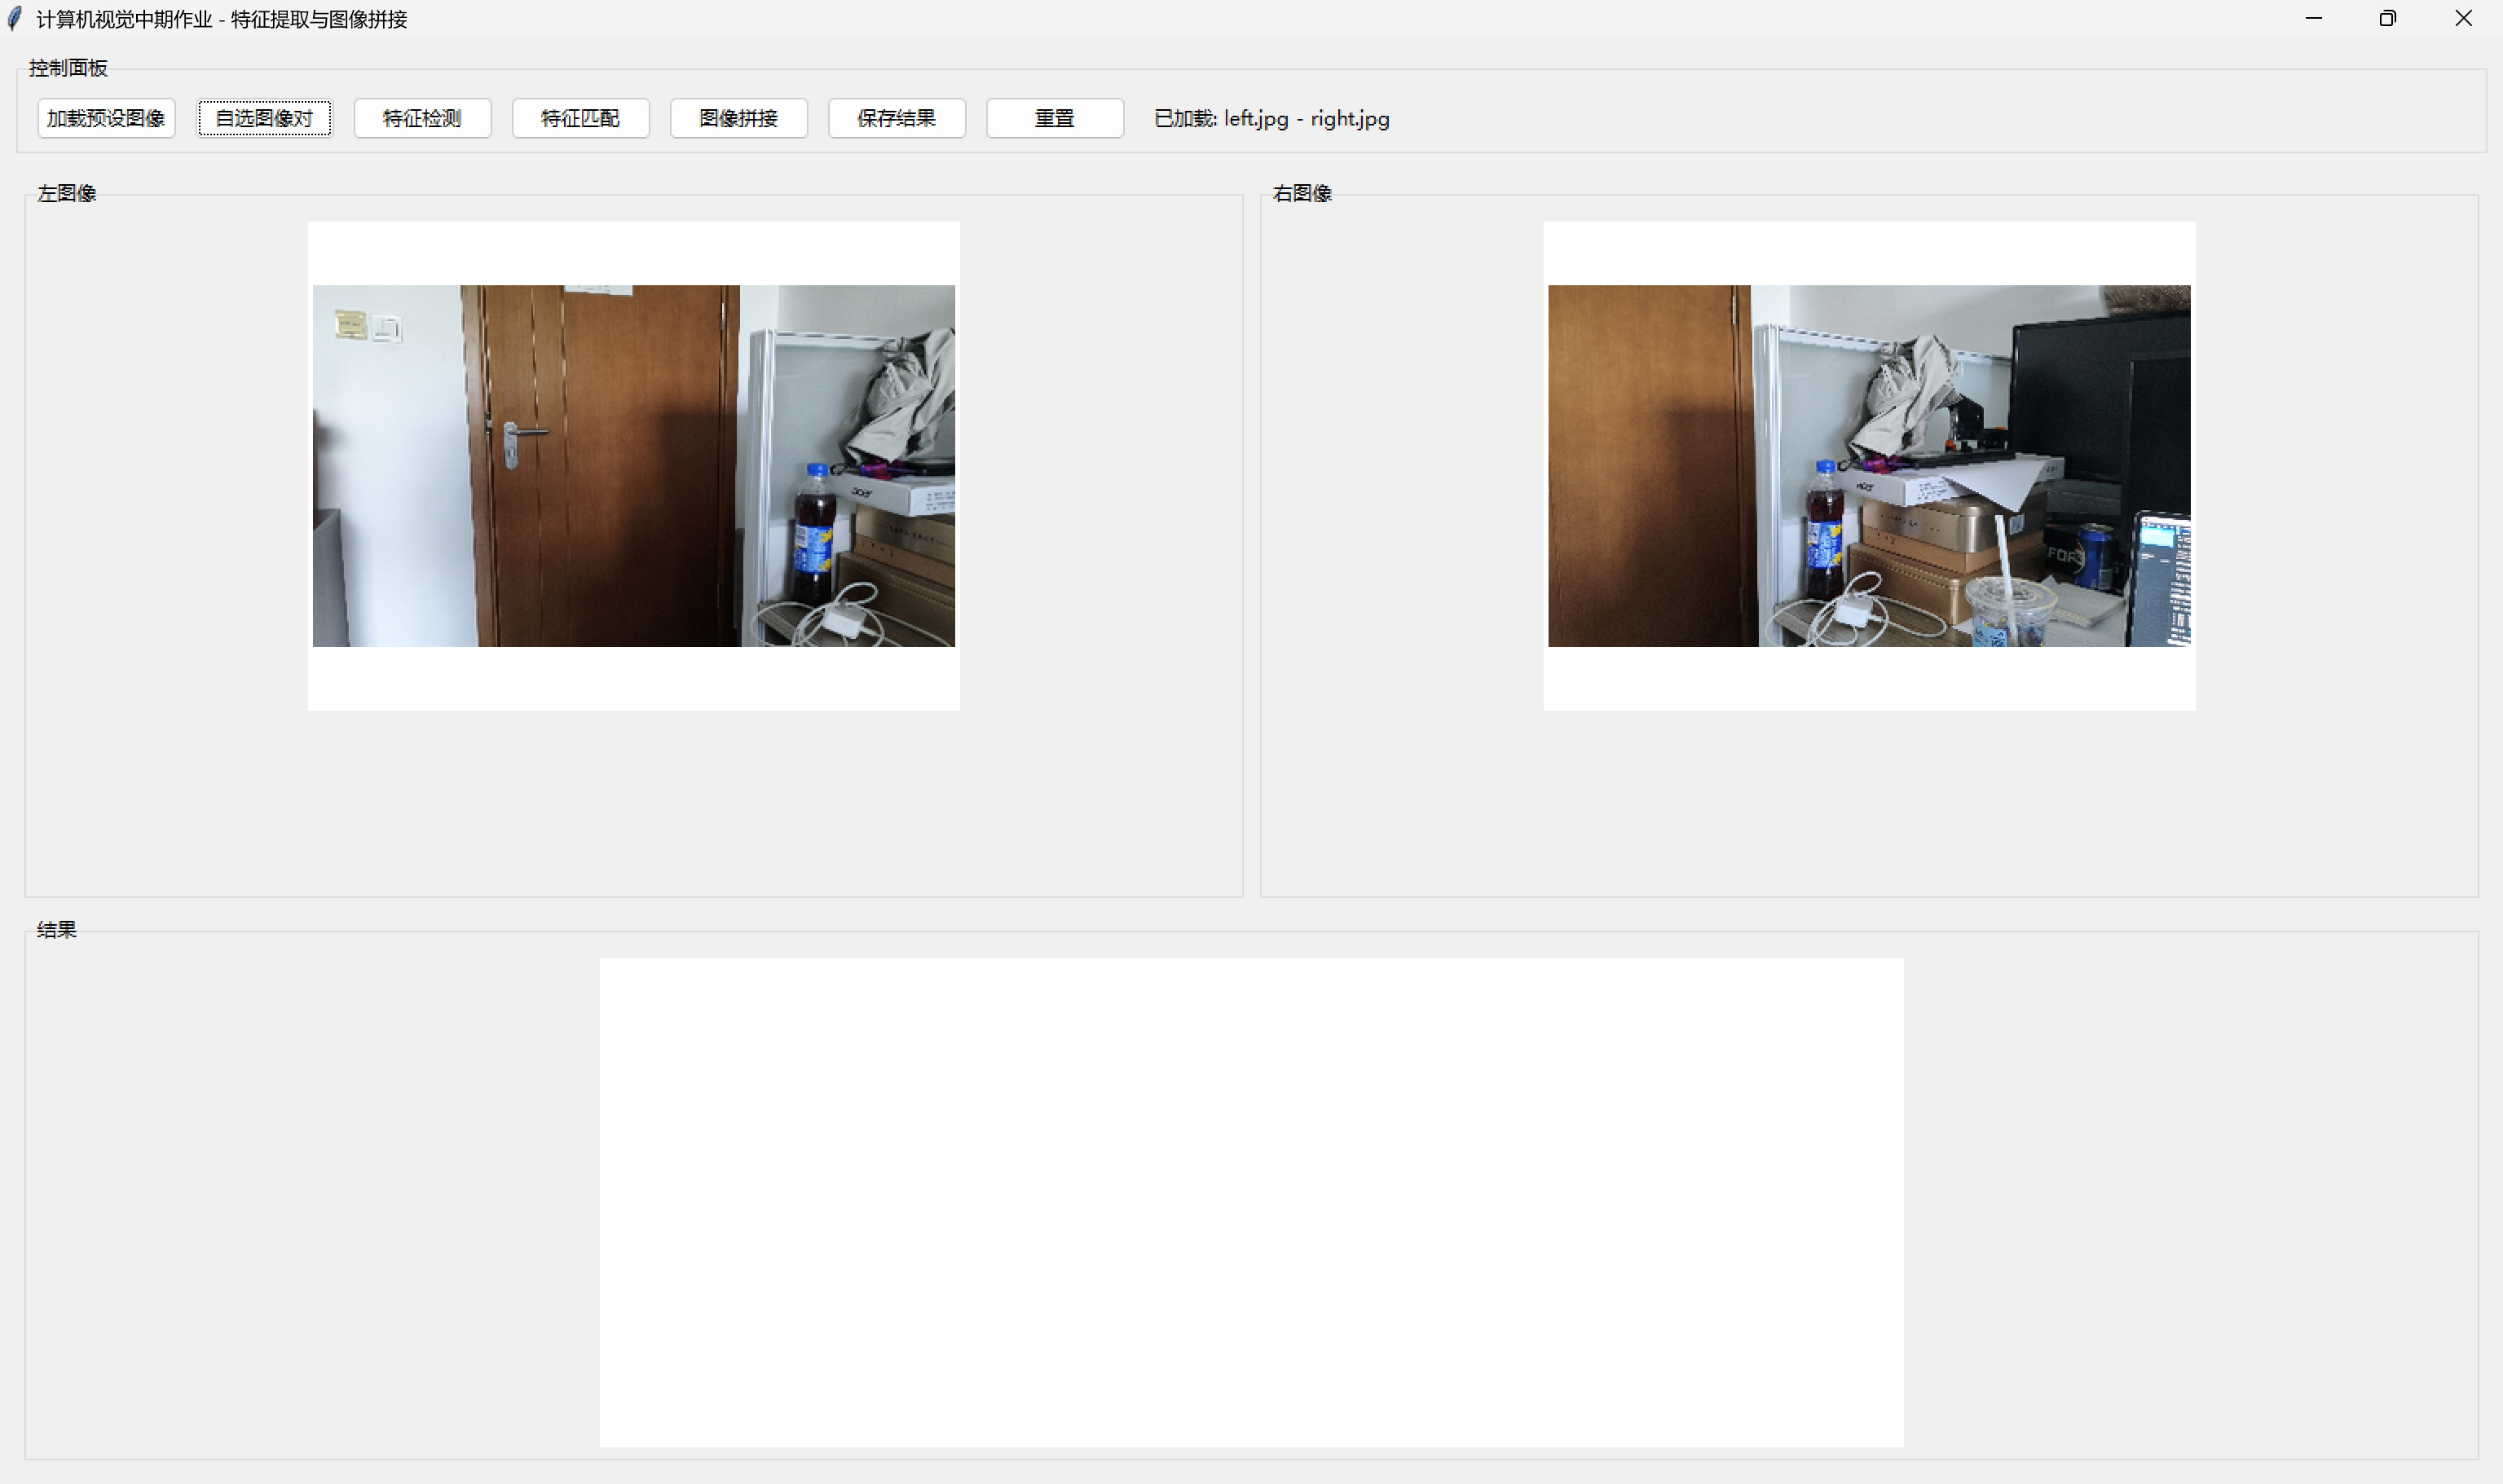
\includegraphics[width=\textwidth]{加载图像.jpg}
\caption{步骤一：通过「自选图像对」加载实拍图像，左右画布分别显示原始图像，状态栏提示已加载文件名}
\label{fig:gui_load}
\end{figure}

\begin{figure}[H]
\centering
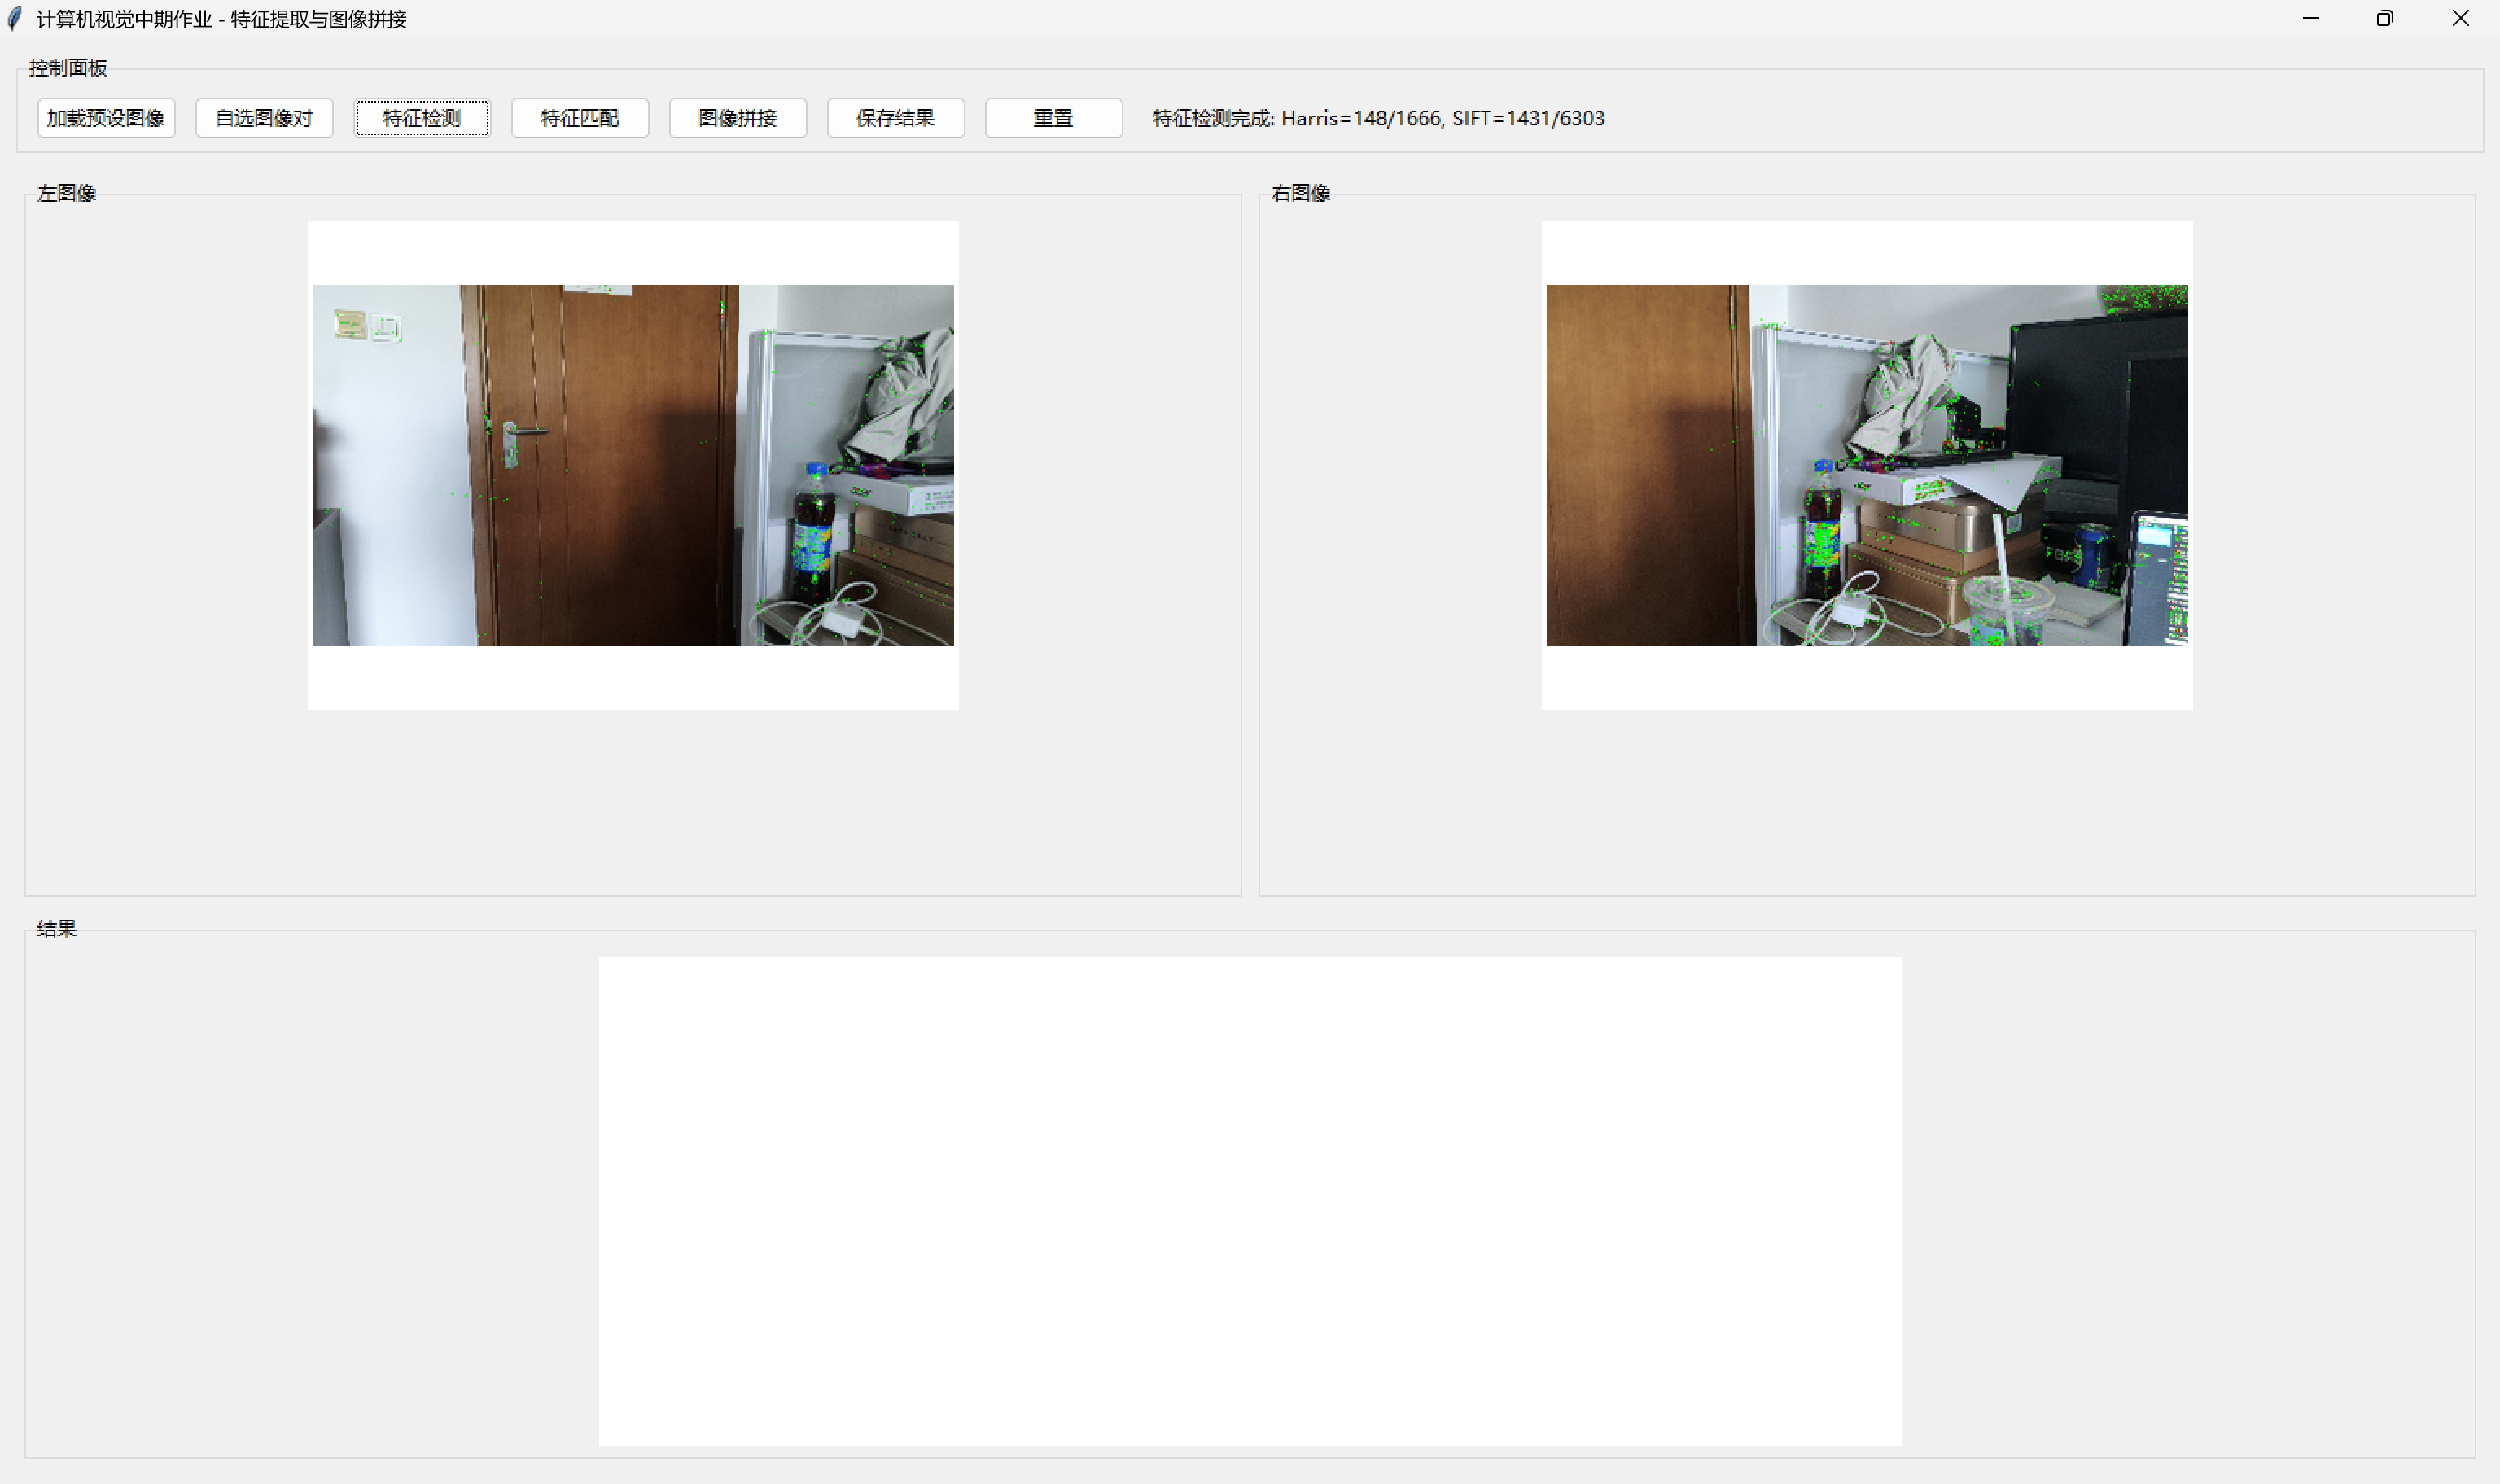
\includegraphics[width=\textwidth]{特征检测.jpg}
\caption{步骤二：特征检测完成后，状态栏显示Harris角点数（148/1666）和SIFT特征点数（1431/6303）}
\label{fig:gui_detect}
\end{figure}

\begin{figure}[H]
\centering
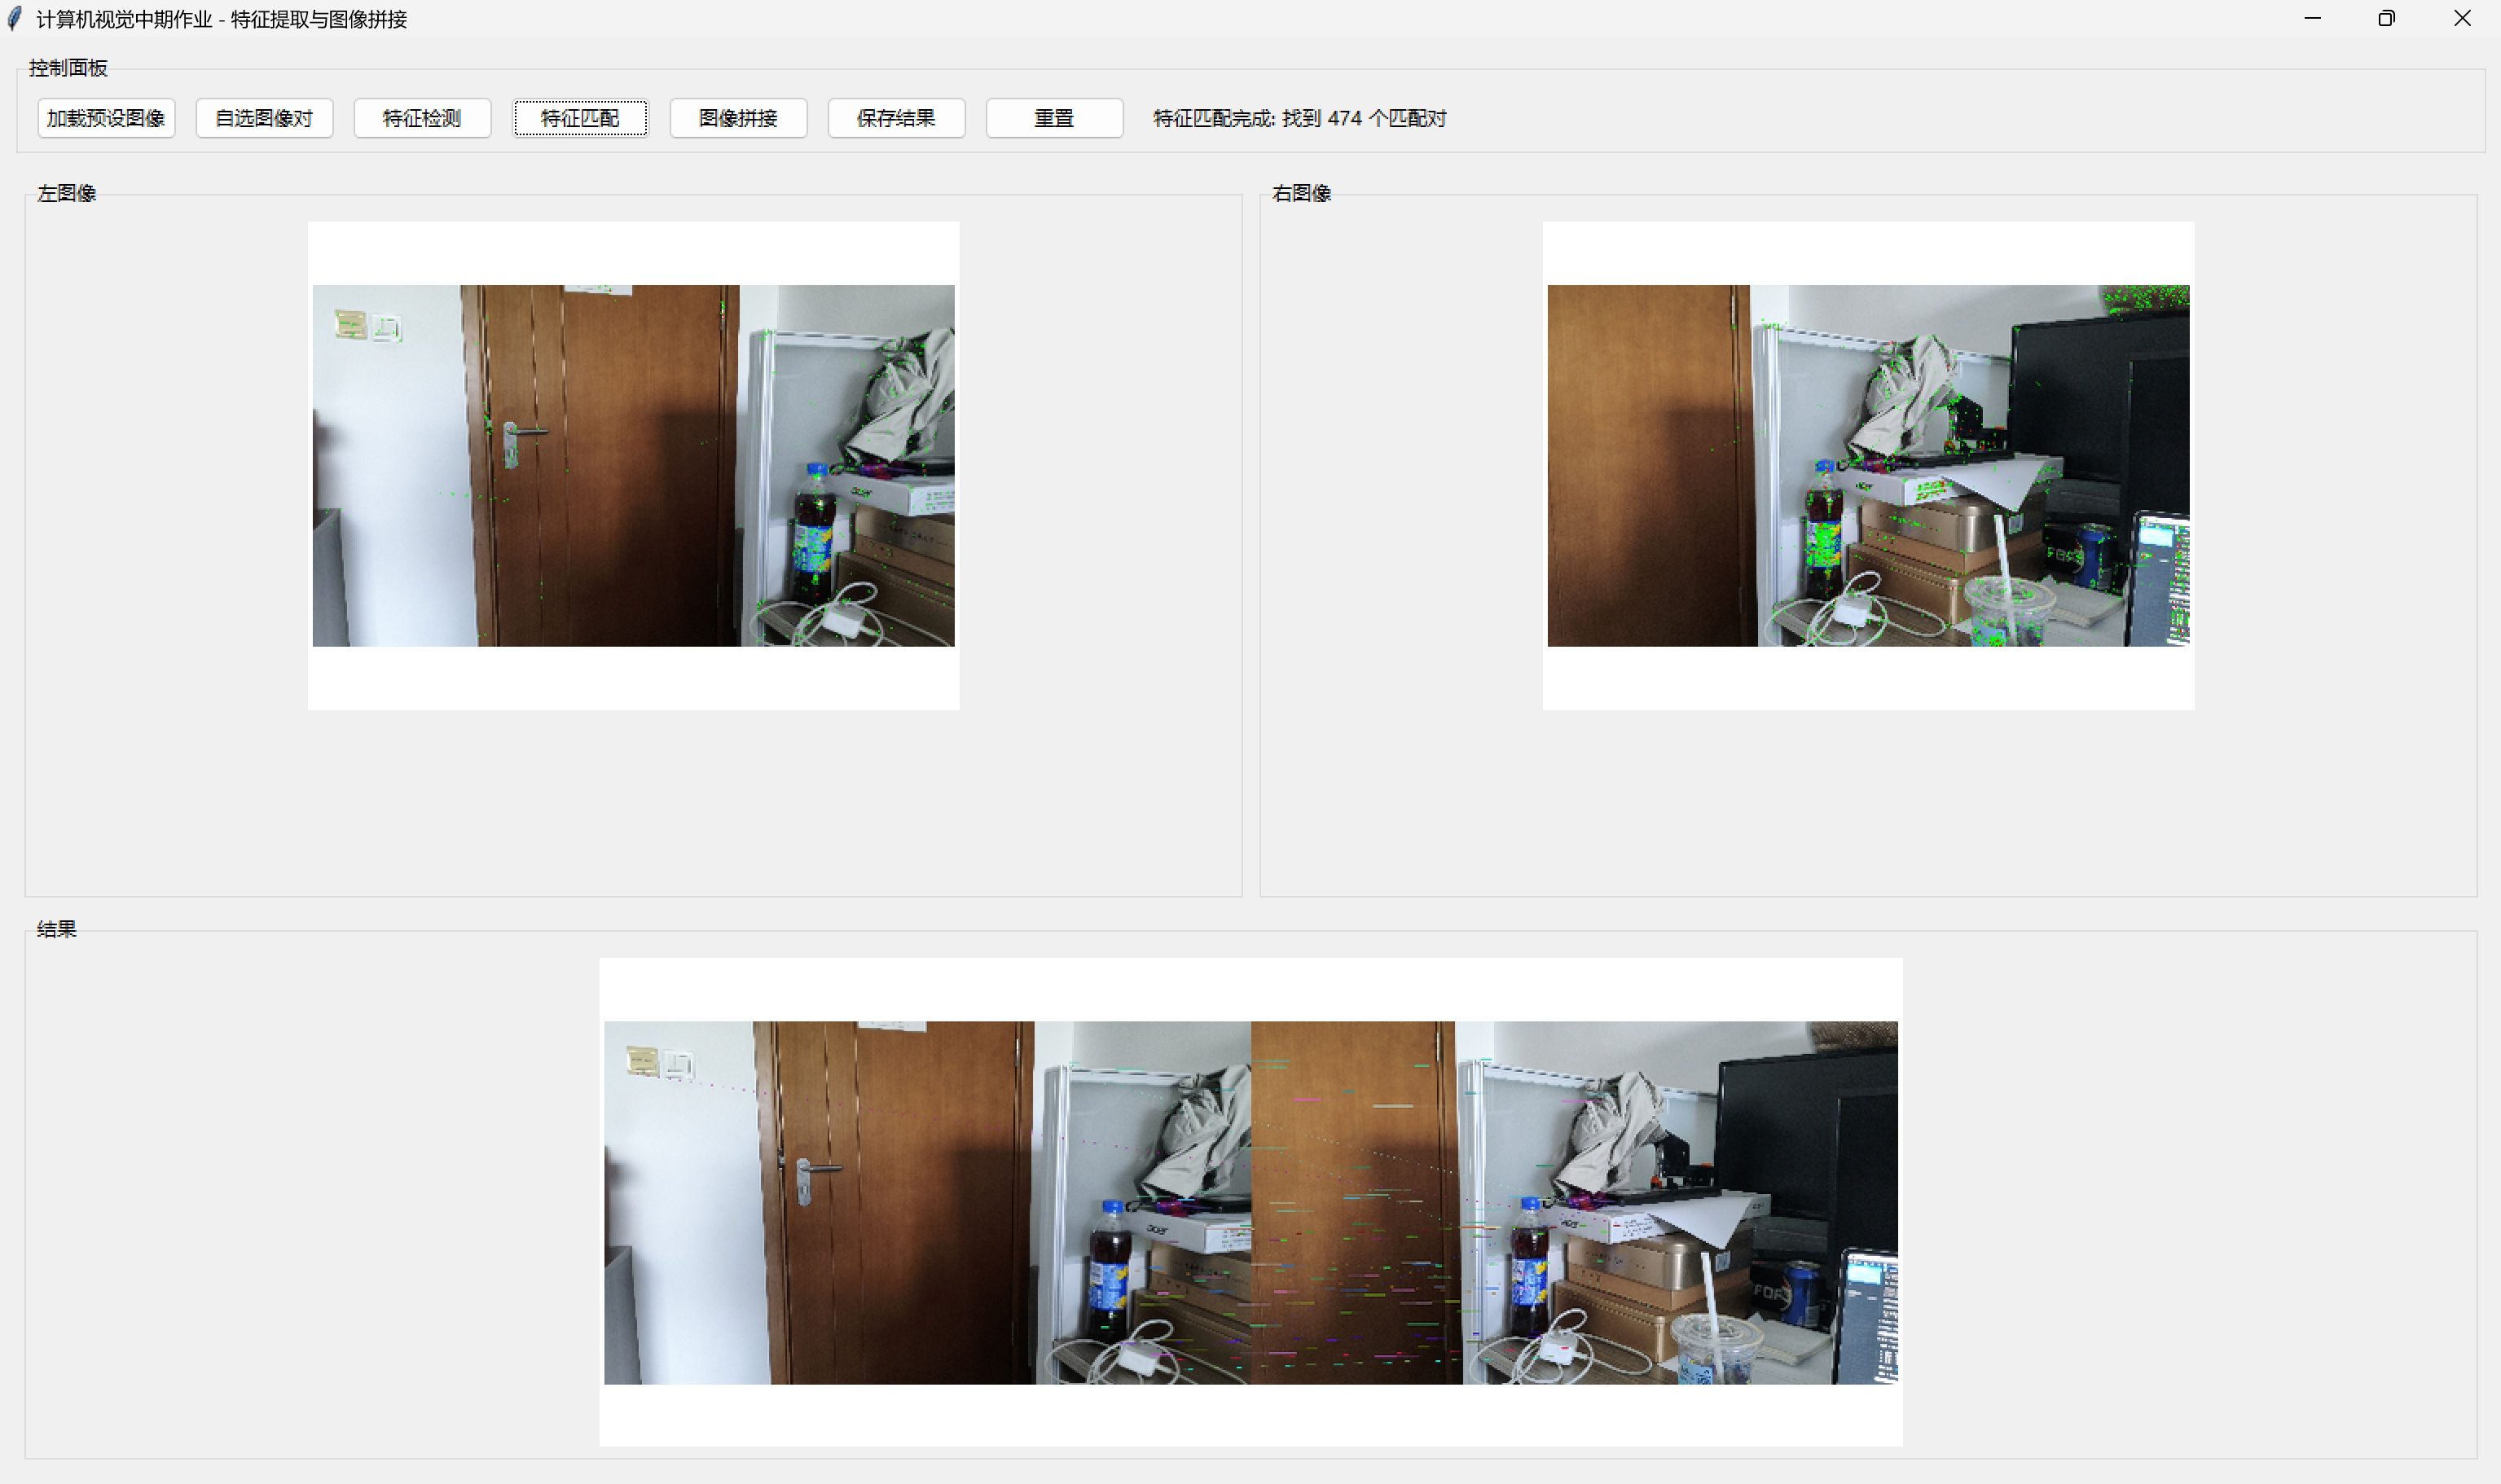
\includegraphics[width=\textwidth]{特征匹配.jpg}
\caption{步骤三：特征匹配完成，状态栏显示找到474个匹配对，底部结果区域以彩色连线展示部分匹配对应关系}
\label{fig:gui_match}
\end{figure}

\begin{figure}[H]
\centering
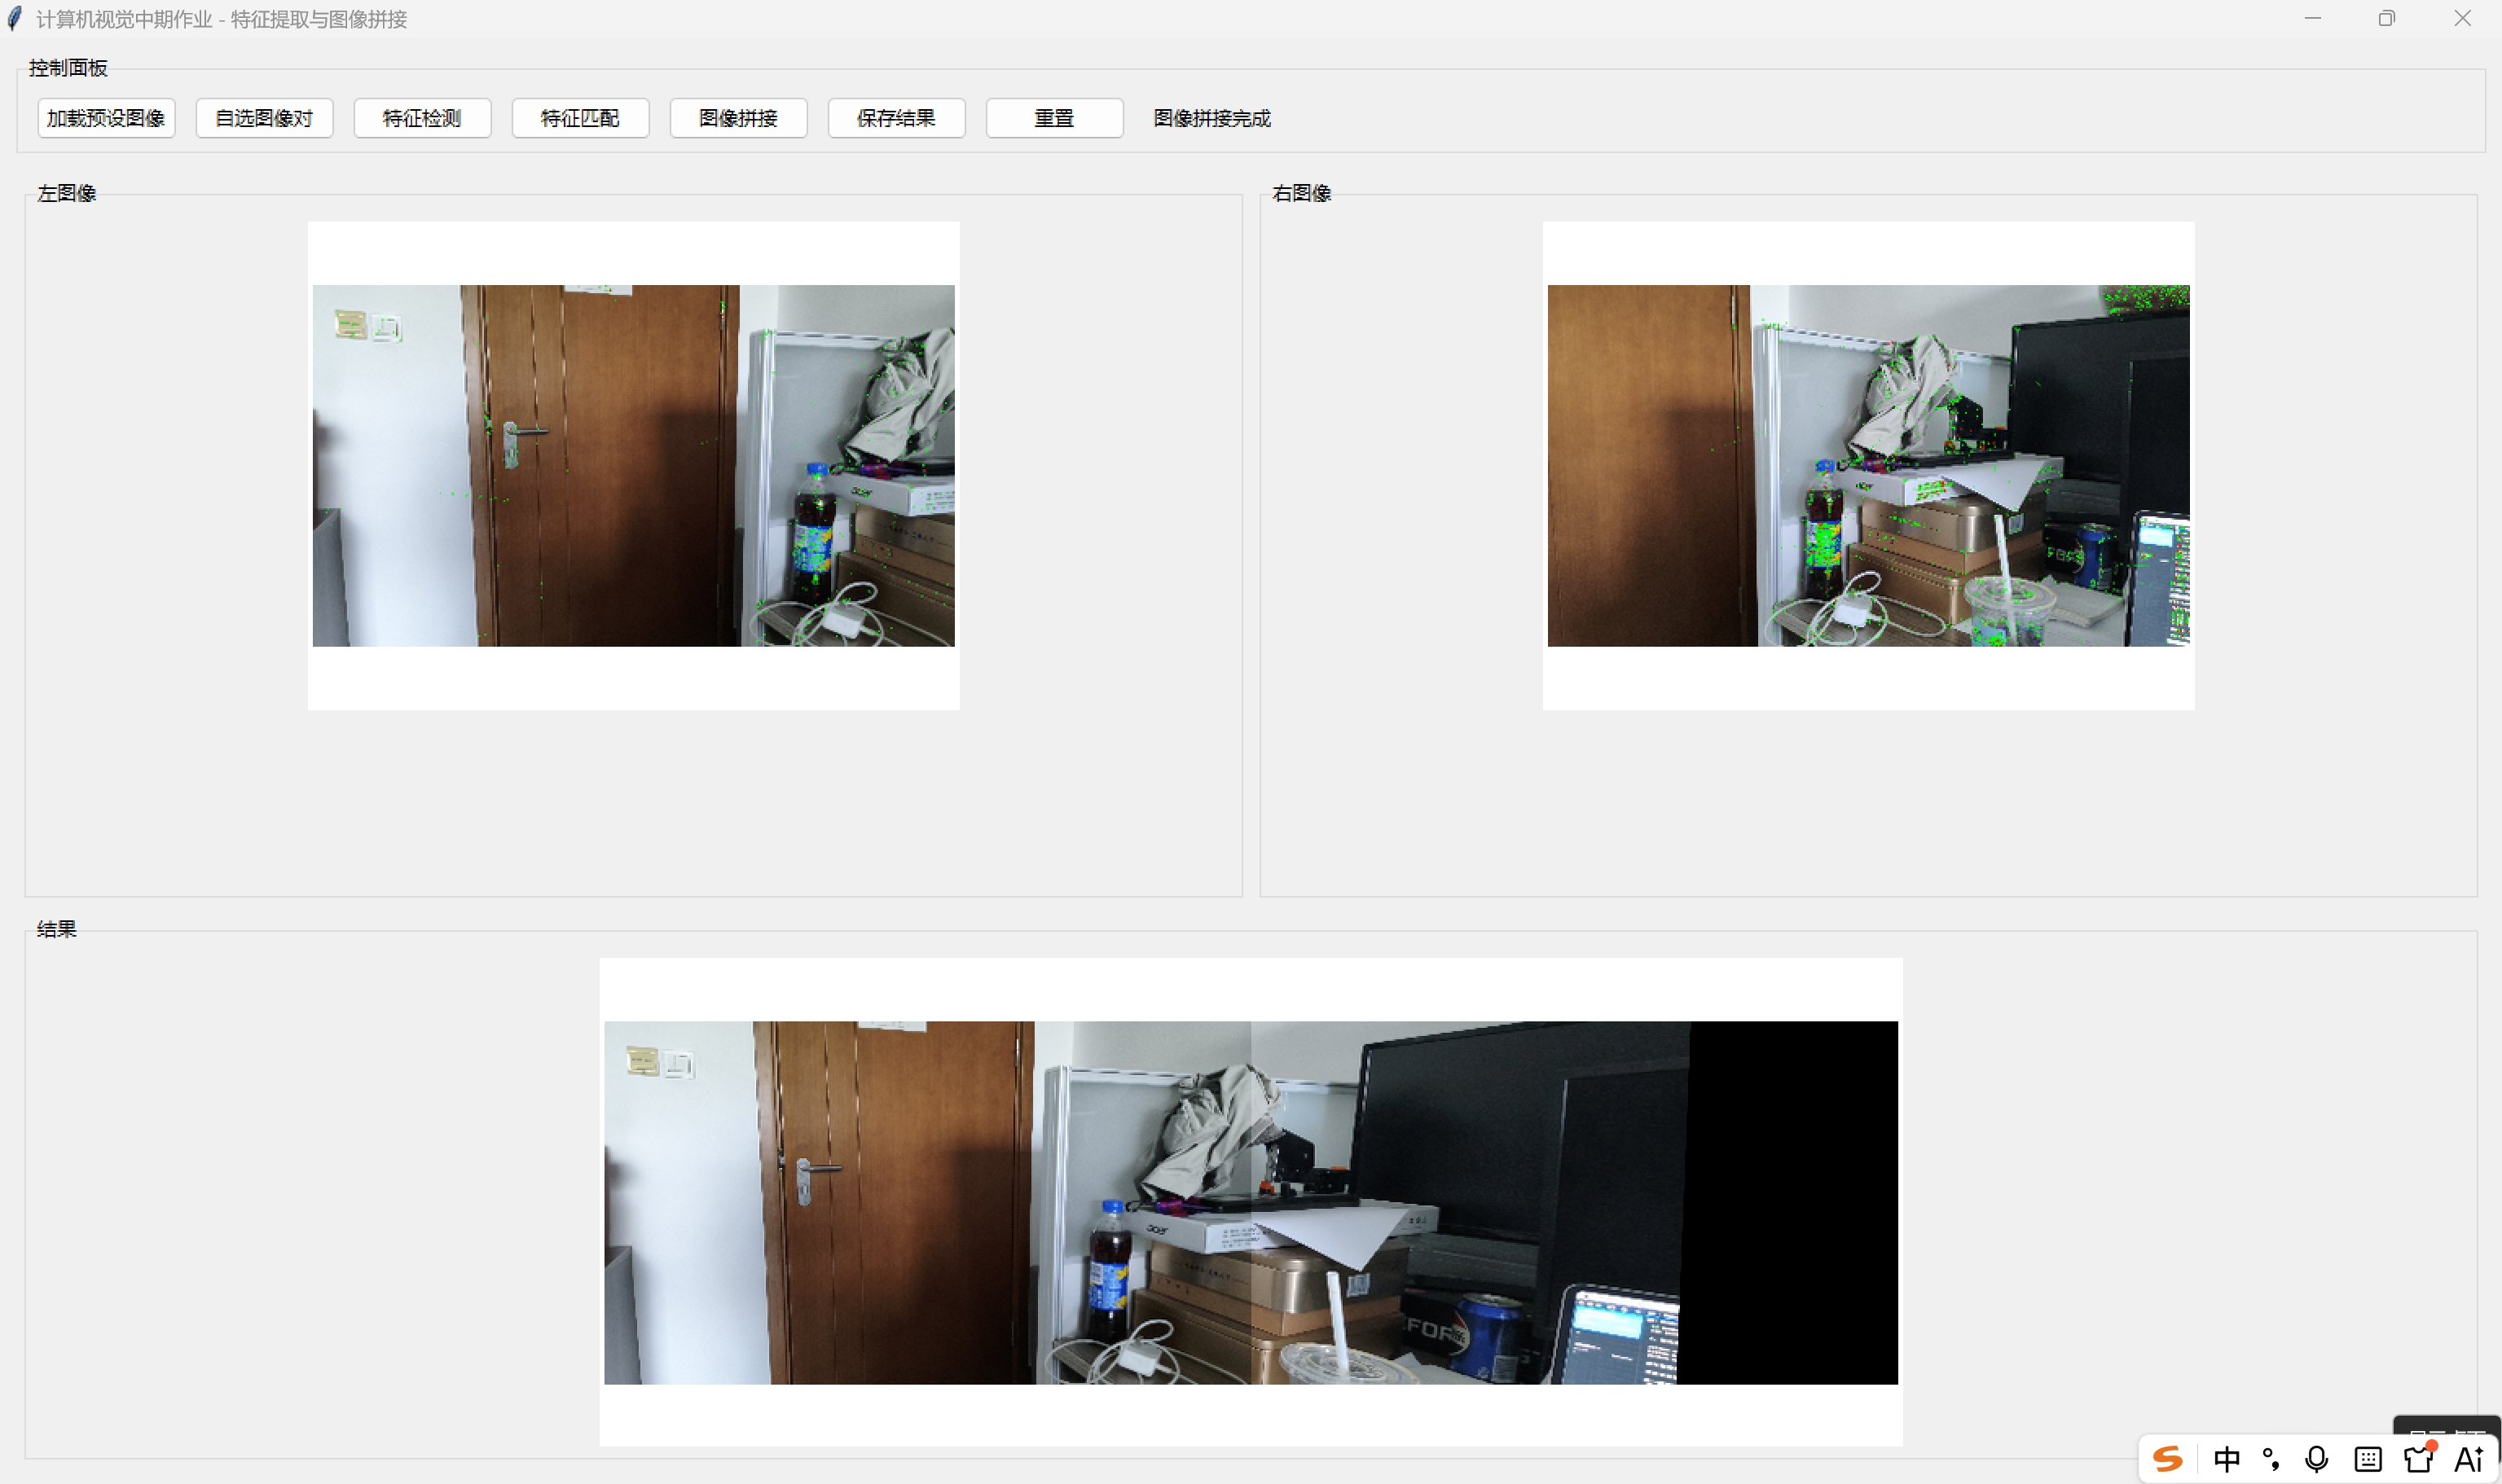
\includegraphics[width=\textwidth]{图像拼接.jpg}
\caption{步骤四：图像拼接完成，底部结果区域显示最终的全景拼接图像，实验室场景被成功拼接为一幅完整的宽幅画面}
\label{fig:gui_stitch}
\end{figure}

从实拍测试结果可以看到，系统在真实的室内手持拍摄场景下仍能正确地完成从特征检测到全景拼接的完整流程。实验室场景中门框等结构提供了丰富的角点和纹理特征，使得SIFT检测到了6303个特征点（右图），Ratio Test匹配后保留了474个高质量匹配对，最终拼接的全景图像自然连贯。

% ============================================================
\section{总结}

本文设计并实现了一个完整的图像特征检测、描述、匹配与全景拼接系统，并在包含9对不同场景的数据集上进行了系统性的实验评估。

在特征检测层面，实验结果表明SIFT在检测数量、空间分布均匀性和特征信息丰富度（尺度与方向）方面全面优于Harris角点检测，尽管后者在计算效率和实现简洁性上具有一定优势。在特征匹配层面，Lowe比值检验的引入被证明是提升匹配质量的关键因素——相比纯SSD最近邻策略，Ratio Test将平均匹配准确率从23\%提升至70\%，同时保留了91\%以上的正确匹配。在描述子选择方面，SIFT的128维浮点描述子在匹配数量和召回率上表现更优，适合对匹配质量要求较高的离线处理场景；ORB的32字节二进制描述子在检测速度上具有7--8倍的优势，更适合实时应用。在图像拼接层面，基于RANSAC的单应性估计对于相机近似纯旋转的场景（如Google Earth街景截图）能够产生优秀的全景图；而对于存在显著相机平移和场景深度变化的情况（如Tanks and Temples室内数据），单应性模型的平面假设被违反，拼接质量出现明显下降，这一发现为理解单应性变换的适用边界提供了直观的实验依据。

\vspace{3em}
\begin{center}
\textbf{最后，感谢老师和助教的辛勤付出！}
\end{center}

\end{document}
